%%%%%%%%%%%%%%%%%%%%%%%%%%%%%%%%%%%%%%%%%%%%%%%%%%%%%%%%%%%%%%%%%%%%%%%%

%%% LaTeX Template for ECAI Papers 
%%% Prepared by Ulle Endriss (version 1.0 of 2023-12-10)

%%% To be used with the ECAI class file ecai.cls.
%%% You also will need a bibliography file (such as mybibfile.bib).

%%%%%%%%%%%%%%%%%%%%%%%%%%%%%%%%%%%%%%%%%%%%%%%%%%%%%%%%%%%%%%%%%%%%%%%%

%%% Start your document with the \documentclass{} command.
%%% Use the first variant for the camera-ready paper.
%%% Use the second variant for submission (for double-blind reviewing).

%\documentclass{ecai} 
\documentclass[doubleblind]{ecai} 

%%%%%%%%%%%%%%%%%%%%%%%%%%%%%%%%%%%%%%%%%%%%%%%%%%%%%%%%%%%%%%%%%%%%%%%%

%%% Load any packages you require here. 

\usepackage{latexsym}
\usepackage{amssymb}
\usepackage{amsmath}
\usepackage{amsthm}
\usepackage{booktabs}
\usepackage{enumitem}
\usepackage{graphicx}
\usepackage{color}

\usepackage{tablefootnote}

\usepackage{todonotes}
\presetkeys%
{todonotes}%
{inline,backgroundcolor=yellow}{}

%%%%%%%%%%%%%%%%%%%%%%%%%%%%%%%%%%%%%%%%%%%%%%%%%%%%%%%%%%%%%%%%%%%%%%%%

%%% Define any theorem-like environments you require here.

\newtheorem{theorem}{Theorem}
\newtheorem{lemma}[theorem]{Lemma}
\newtheorem{corollary}[theorem]{Corollary}
\newtheorem{proposition}[theorem]{Proposition}
\newtheorem{fact}[theorem]{Fact}
\newtheorem{definition}{Definition}

%%%%%%%%%%%%%%%%%%%%%%%%%%%%%%%%%%%%%%%%%%%%%%%%%%%%%%%%%%%%%%%%%%%%%%%%

%%% Define any new commands you require here.

\newcommand{\BibTeX}{B\kern-.05em{\sc i\kern-.025em b}\kern-.08em\TeX}

%%%%%%%%%%%%%%%%%%%%%%%%%%%%%%%%%%%%%%%%%%%%%%%%%%%%%%%%%%%%%%%%%%%%%%%%

\begin{document}
	\newcommand{\samenote}{\footnotemark[1]} 
	
	%%%%%%%%%%%%%%%%%%%%%%%%%%%%%%%%%%%%%%%%%%%%%%%%%%%%%%%%%%%%%%%%%%%%%%%%
	
	\begin{frontmatter}
		
		%%% Use this command to specify your submission number.
		%%% In doubleblind mode, it will be printed on the first page.
		
		\paperid{123} 
		
		%%% Use this command to specify the title of your paper.
		
		\title{GLOVE-ITE: Compact Variational Autoencoder for Treatment Effect Estimation with Irrelevant Variables
			%\todo[author=jsk]{Is the VAE compact (as in the model is small and has few weights) or is the latent space compact, or are we using a small part of the latent space in downstream tasks? Are we learning compact latent spaces for TEE with Irrelevant Variables?}
		}
		
		%%% Use this combinations of commands to specify all authors of your 
		%%% paper. Use \fnms{} and \snm{} to indicate everyone's first names 
		%%% and surname. This will help the publisher with indexing the 
		%%% proceedings. Please use a reasonable approximation in case your 
		%%% name does not neatly split into "first names" and "surname".
		%%% Specifying your ORCID digital identifier is optional. 
		%%% Use the \thanks{} command to indicate one or more corresponding 
		%%% authors and their email address(es). If so desired, you can specify
		%%% author contributions using the \footnote{} command.
		
		\author[A]{\fnms{A}~\snm{A}\thanks{Corresponding Author. Email: somename@university.edu.}}
		
		\author[A]{\fnms{B}~\snm{B}}
		
		\author[A]{\fnms{C}~\snm{C}} 
		
		\address[A]{U}
		
		
		%\author[A]{\fnms{First}~\snm{Author}\orcid{....-....-....-....}\thanks{Corresponding Author. Email: somename@university.edu.}\footnote{Equal contribution.}}
		%\author[B]{\fnms{Second}~\snm{Author}\orcid{....-....-....-....}\footnotemark}
		%\author[B,C]{\fnms{Third}~\snm{Author}\orcid{....-....-....-....}} 
		
		%\address[A]{Short Affiliation of First Author}
		%\address[B]{Short Affiliation of Second Author and Third Author}
		%\address[C]{Short Alternate Affiliation of Third Author}
		
		%%% Use this environment to include an abstract of your paper.
		
		%%%%%%%%%%%%%%%%%%%%%%%%%%%%%%%%%%%%%%%%%%%%%%%%%%%%%%%%%%%%%%%%%%%%%%%%
		
		\begin{abstract}
			Estimating treatment effects from imbalanced observational data is crucial in many fields of science and many state-of-the-art methods use Variational Autoencoders (VAEs) for learning a balanced data representation of predetermined width. However, width mismatch easily leads to over- or underfitting of outcome prediction because too little relevant or too much irrelevant information is encoded. As manually determining width by cross-validation is impractical for many current models and for large data sets with irrelevant variables, approaches that automatically determine the size are needed. 
			%
			In this paper, we learn sparsity-inducing masks that sub-select dimensions for each prediction task to automatically determine the effective width of the representation. To achieve this, we use a differentiable $L_0$ sparsity objective that penalizes non-zero elements in the masks. We manage the trade-off between the conflicting objectives with prioritization and optimize sparsity only when prediction passes a threshold, using the Generalized ELBO with Constrained Optimization (GECO) framework.
			%
			Our method accurately infers latent factors relevant to treatment effect estimation, resulting in a compact representation and the learned masks successfully isolate irrelevant variables in the challenging high-dimensional data.
			%
			We show favorable results for both real-world and synthetic datasets with increasing numbers of irrelevant variables, providing better predictive accuracy, compactness of the latent space, and disentanglement of latent factors. 
		\end{abstract}
	\end{frontmatter}
	\section{Introduction}
	
	Treatment effect estimation is a challenging task that involves latent factors and mitigating selection bias to achieve robust and accurate estimations \citep{PaulRD,ganite}. Traditional propensity score-based methods \citep{PaulRD,PaulR,Sheng} to remove selection bias often struggle to deliver, particularly in large feature spaces, where the complexity of relationships between covariates and outcomes poses major challenges.
	
	
	%\todo[author=jsk]{Mention why people are using propensity score methods: for balancing which removes the selection bias.}
	
	%\todo[author=jsk]{Why does it involve identifying latent factors? It is because we want to do causal reasoning? Do we identify them in order to mitigate selection bias? Do not already get the factors sorted by what they are supposed to be doing? What is the scenario?
		
		%What are these traditional approaches? Statistics or ML? Can we give more details how they fail?}
	
	In contrast, deep neural network-based approaches \citep{Johansson,UriSha,SITE,Negar_2} have emerged as a compelling choice, especially in high-dimensional and large data settings. These methods learn balanced intermediate representations, enabling more precise predictions for the downstream prediction tasks associated with treatment effect estimation. Specifically, VAE-based approaches  \citep{CEVAE,TEDEV,vowels2021targeted} have been used to learn smooth and disentangled representations at the bottleneck. These methods utilize separate inference networks and optimize a joint objective consisting of reconstruction, treatment prediction, and outcome prediction which together minimize selection bias in the learned latent space.
	
	However, a key issue in existing VAE-based approaches is predefined bottleneck width, i.e.\ the number of dimensions for representation of the latent factors. An overly large width can lead to overfitting, higher reconstruction error and spurious correlations between latent variables, while an insufficient width risks underfitting. Both cases undermine the accuracy of the target task \citep{bonheme2023the}. Although cross-validation is a widely used solution, it is computationally expensive and impractical for large data sets. This issue becomes even more pronounced in large models with multiple encoders and irrelevant variables, where each encoder is tasked with representing a distinct latent factor. In treatment effect estimation, suboptimal bottleneck width can lead to inaccurate inference of latent factors, resulting in spurious treatment effect estimates. We showcase this issue in our results in Table \ref{tab:IHDP} and Figure \ref{fig:learning_curves}.
	%
	Furthermore, the presence of irrelevant variables in large-scale observational data is inevitable, and failure to explicitly account for them can bias the learned representation and ultimately degrade the accuracy of treatment effect estimation \citep{Khan2024OnTE}.
	
	\begin{comment}
		\todo[author=jsk]{So-far the bottleneck size and over / under fitting seem to behave exactly like the number of network parameters when it comes to over / under fitting. We need to more clearly state why we are interested in the bottleneck. Is it because we want to really identify the causal factors or because we want to know something about the data?
			
			We should also comment on the fact that VAE is supposed to find this bottleneck automatically but does not or cannot. Do we know why? Is the reconstruction task conflicting with the TEE task?
			
			There are also models with huge latent spaces (or intermediate layers) like the Johansson papers. How do we position ourselves towards them? Are they just wrong? Are they solving a different problem? Why do they not use a bottleneck? Is there a benefit to using a bottleneck that they do not make use of?
			
			Who is helped by knowing the best bottleneck dimension? The downstream user?
		}
	\end{comment}
	
	
	%In this paper, we propose a novel VAE-based framework that simultaneously learns the latent space dimensionality for each latent factor instead of relying on a pre-defined or iteratively tuned values and estimates treatment effects.
	
	In this paper, we propose a novel VAE-based framework that jointly estimates treatment effects and automatically determines the dimensionality of the latent representation by inducing sparsity in the VAE bottleneck which eliminates the need for pre-defined or manually tuned bottleneck width. For this, we use a differentiable $L_0$ objective on the VAE bottleneck using a sparsity-inducing mask \citep{louizos2018learning}.
	%
	However, optimizing bottleneck sparsity without constraints as part of the joint objective is detrimental as shown in our results (Figure \ref{fig:learning_curves}). For this reason, we use Generalized ELBO with Constrained Optimization (GECO) \citep{JimenezRezende2018TamingV,Boom2020DynamicNO} which allows us to prioritize the prediction task over sparsity.
	%
	Additionally, to address the challenge of irrelevant variables in data, our method learns a dedicated mask that separates irrelevant factors into a distinct latent subspace, thereby enhancing robustness in treatment effect estimation.
	To the best of our knowledge, no existing method combines $L_0$ regularization with GECO to optimize the VAE bottleneck for treatment effect estimation. 
	
	Our approach demonstrates superior performance compared to state-of-the-art VAE-based methods on the Infant Health and Development Program (IHDP) dataset as well as a challenging synthetic dataset \citep{Gunn,Hill,Khan2024OnTE}. We further provide valuable qualitative insights into our framework, enhancing its practicality and stability for real-world applications. 
	%\todo[author=jsk]{Reference for the dataset}
	The core contributions of our work are as follows:
	%
	\begin{itemize}
		%
		\item We introduce a novel VAE-based framework that integrates GECO and $L_0$ regularization to automatically learn sparsity masks for each latent factor while ensuring constraint satisfaction, improving robustness in treatment effect estimation.
		
		\item Our approach effectively addresses irrelevant variables by introducing a learnable mask and a dedicated latent subspace, leading to improved accuracy in treatment effect estimation.
		
		\item We provide a shared and compact encoder architecture to efficiently learn distinct latent factor representations, enhancing disentanglement. These advancements are validated through extensive qualitative analysis on real-world and synthetic datasets.
		
		
		
	\end{itemize}
	
	
	
	%\todo[author=jsk]{Make sure that all of the bullet points use the same mode of speech. Is the partitioned encoder a contribution? Should the extensive evaluation with the synthetic dataset and the permutation analysis be mentioned here?}
	
	\section{Related Work}
	\label{sec:related-work}
	
	%\todo[author=jsk]{If possible, connect this text more closely to this paper. Use phrases like
		
		%- Similar to ... we do ...
		
		%- Different to .. we do ...
		
		%- In contrast to ... we do ...
		
		%and so on}
	
	Selection bias is a well-known challenge in treatment effect estimation \citep{PaulRD}, traditionally addressed through propensity score-based techniques like matching, stratification, and re-weighting \citep{PaulRD,PaulR,Sheng}. However, these methods have limited effectiveness in high-dimensional real-world scenarios \citep{conf}. For high-dimensional settings, deep representation learning approaches have emerged as a powerful alternative for balancing individual samples \citep{Johansson,UriSha,SITE,Negar_2}. These methods aim to mimic a Randomized Controlled Trial (RCT) by reducing bias between treatment groups in a joint embedding space for all variables. However, they fail to consider that not all covariates typically contribute to both the treatment and the outcome.
	
	In contrast, disentanglement approaches further advance this idea by additionally separating instrumental, confounding, and adjustment factors to better capture underlying causal structures and have proved effective in addressing selection bias \citep{Decomp,Negar,kuang2020data,Anpeng,Ortho}. Here, the latent space is often learned with variational autoencoders, e.g.\ focussing solely on confounding factors \citep{CEVAE} or separating all three latent factors \citep{TEDEV}.
	
	However, separating out irrelevant factors is highly relevant for treatment effect estimation because they can lead to spurious effect estimation and it was observed that higher number of irrelevant dimensions make state-of-the-art approaches fail \citep{Khan2024OnTE}. Therefore, models with four separate encoders and suitable loss functions have been suggested to deal with irrelevant factors \citep{vowels2021targeted,Khan2024OnTE}. 
	
	Despite their strengths, deep disentanglement and VAE-based approaches are sensitive to the number of latent factor dimensions, making determining the right latent dimensionality crucial to performance and avoiding spurious treatment effect estimates. Existing methods for this often rely on the elbow method or expensively training multiple models \citep{Mai,doersch2021tutorialvariationalautoencoders,FONDUE}.
	%
	
	In contrast to tedious and expensive search for suitable bottleneck dimensionality, we propose a novel VAE-based solution leveraging  a $L_0$ sparsity and constrained optimization objective.  This approach is connected to intrinsic dimension estimation, which identifies effective latent size needed to describe data and has been explored for other deep learning tasks \citep{Levina2004MaximumLE,Facco2017EstimatingTI,Gong2018OnTI,Ansuini2019IntrinsicDO,pope2021intrinsic}. 
	%Applications in deep learning reveal that image IDs are much lower than their pixel dimensions and that neural networks with strong generalization exhibit decreasing ID estimates in the final layers \cite{Gong2018OnTI,Ansuini2019IntrinsicDO,pope2021intrinsic}. 
	%In contrast, FONDUE \cite{FONDUE} identifies redundant dimensions by detecting divergences in intrinsic dimensionality between mean and sampled representations during training. However, these methods involve a resource-intensive process that requires fully training multiple models, significantly increasing both the computational cost and the environmental impact of experiments.
	%
	Finally, the way \citet{Boom2020DynamicNO} induces sparsities in VAE bottlenecks unrelated to the treatment effect estimation problem serves as an inspiration for this work. Yet our $L_0$ sparsity objective is less computationally involved and e.g. does not require several forward passes for each data point. 
	
	%theoretically aligns with our approach, their method addresses the classic VAE bottleneck problem through reconstruction loss constraints and is not designed for multi-encoder downstream tasks. Furthermore, their implementation of $L_0$ regularization is computationally intensive compared to our streamlined solution.
	
	
	
	
	%\todo[author=jsk]{The following might better be integrated to the intro?}
	
	
	%\todo[author=jsk]{Up to here, all related work is about TEE. We should also discuss that bottleneck dim. determination is often not seen as a problem in VAEs and what the recommended practical approach is. Then we can give some references how this works.}
	
	
	
	\section{Background Knowledge}
	\label{sec:background}
	
	In this section, we provide a cursory explanation of the Treatment Effect Estimation problem and the Variational Autoencoder (VAE) model. 
	
	\subsection{Treatment Effect Estimation}
	\label{sec:background-tee}
	
	%separating instrumental ($\Gamma$: influence treatment selection), confounding ($\Delta$: affect both treatment selection and outcome), and adjustment ($\Upsilon$: impact outcome only)
	
	An observational datasets $\mathcal{D} = \{ \mathbf{x}^{(i)}, t^{(i)}, y^{(i)}\}_{i=1}^N$ consists of pre-treatment variables $\mathbf{x}^{(i)} \in \mathcal{X} \subseteq \mathbb{R}^K$, treatments $t^{(i)} \in \mathcal{T}$ (e.g., {0: medication, 1: surgery}), and observed outcomes $y^{(i)} \in \mathcal{Y}$ (e.g., recovery time). 
	%
	However, only the factual outcomes $y^{t(i)}$ are observed, while the counterfactual outcomes $y^{\neg t (i)}$ remain unobserved. 
	%
	Selection bias is present when treatment assignment depends on $\mathbf{x}^{(i)}$, violating the randomized controlled trial assumption $P(\mathcal{T} \mid \mathcal{X}) = P(\mathcal{T})$. 
	%
	The objective is to estimate the Individual Treatment Effect (ITE), defined as $ \mathrm{ite}_{i} = y^{1(i)} - y^{0(i)}$, by learning a function $f \colon \mathcal{X} \times \mathcal{T} \to \mathcal{Y}$ \citep{Negar,Khan2024OnTE}.
	
	\begin{equation}
		\widehat{\text{ite}}_i =
		\begin{cases}
			y^{1(i)} - f(\mathbf{x}^{(i)}, 1 - t^{(i)}), & \text{if } t^{(i)} = 1 \\
			f(\mathbf{x}^{(i)}, 1 - t_i) - y^{0(i)} ), & \text{if } t^{(i)} = 0
		\end{cases}
	\end{equation}

	
	 Treatment effect estimation relies on the following widely adopted assumptions \citep{PaulRD,assumptions,Imbens}. %We additionally posit the following common assumptions%. Treat
	%
	\begin{itemize}
		\item \textbf{Stable Unit Treatment Value:} The treatment assigned to one unit does not influence the potential outcomes of any other unit (i.e. patient).
		%\todo[author=jsk]{Do we know that the reader knows what a unit is?}
		\item \textbf{Unconfoundedness:} There are no unmeasured confounders; all factors affecting both the treatment $\mathcal{T}$ and the outcome $\mathcal{Y}$ have been observed, formally, $\mathcal{Y} \perp\!\!\!\perp \mathcal{T} \mid \mathcal{X} $.
		
		\item \textbf{Overlap:} The probability of receiving any treatment given covariates $\mathbf{x}$ is strictly positive for all treatments.. Formally, $P({t} \mid \mathbf{x}) > 0  \, \forall t \in \mathcal{T}, \forall \mathbf{x} \in \mathcal{X} $ \citep{Rubin}.
		\item \textbf{Consistency:} Let \( y^t \) denote the potential outcome under treatment \( t \in \{0, 1\} \), and let \( \mathcal{T} \) be the actual treatment received. The consistency assumption states that the observed outcome \( y \) equals the potential outcome corresponding to the treatment actually received:
		
		\[
		y = y^t \quad \text{if } \mathcal{T}  = t
		\]
	\end{itemize}
	%
	Aside from selection bias, ITE estimation is further complicated by entangled pre-treatment variables, meaning that instrumental ($\Gamma$: influence treatment selection), confounding ($\Delta$: affect both treatment selection and outcome), adjustment ($\Upsilon$: impact outcome only) variables are not separated in $\mathcal{X}$. In high-dimensional settings, irrelevant variables ($\Omega$) are increasingly prevalent. Their inclusion and entanglement with relevant pre-treatment variables induce spurious dependencies, biasing the learned representations and leading to inaccurate treatment effect estimates if not explicitly handled \citep{Decomp,Khan2024OnTE} as seen in Table \ref{tab:IHDP} below.
	
	
	%\todo[author=jsk]{Note: in the previous paper be made a big argument about that irrelevant factors naturally occur in large scale data collection studies etc. and that they are a very important problem. We should also make the same argument here and in the intro. You can copy the text from the previous paper.}
	
	
	%\todo{Note: Only multidimensional objects are bold. Letters use mathbf and greek symbols use boldsymbol. (boldsymbol is actually not a bold font but a trick to make the symbol appear bold by printing it several times and often looks strange.)}
	
	\subsection{Variational Autoencoders}
	\label{sec:background-vae}
	
	Variational Autoencoders (VAEs) \citep{VAE} are deep generative models with a latent representation bottleneck. %They model the observed data $\mathbf{x}$ as arising from latent variables $\mathbf{z}$ through a probabilistic framework. 
	The generative process uses a prior distribution over the latent variables, $p(\mathbf{z})$ (commonly a Gaussian $\mathcal{N}(0, \mathbf{I})$, and a likelihood function $p(\mathbf{x} \mid \mathbf{z})$, parameterized by a neural network. The objective is to maximize the marginal likelihood
	$ p(\mathbf{x})  =  \int p(\mathbf{x} | \mathbf{z}) p(\mathbf{z}) d\mathbf{z}$, which is generally intractable.
	%
	Instead, we optimize the Evidence Lower Bound (ELBO) on the marginal likelihood,
	%
	\begin{equation}
		\mathcal{L}_{\text{ELBO}} 
		= 
		\mathbb{E}_{q(\mathbf{z}|\mathbf{x})} [\log p(\mathbf{x} | \mathbf{z})] - \text{KL}(q(\mathbf{z}|\mathbf{x}) \| p(\mathbf{z})),
		\label{eq:elbo}
	\end{equation}
	%
	where $q(\mathbf{z} | \mathbf{x})$ is the learned variational posterior (encoder) that approximates the true posterior $p(\mathbf{z} | \mathbf{x})$. The reconstruction loss in the expectation ensures that the latent representation preserves sufficient information and the Kullback-Leibler (KL) divergence induces a structured and smooth latent space.
	%
	The encoder maps $\mathbf{x}$ to the parameters of a Gaussian
	%
	\begin{equation}
		q(\mathbf{z}|\mathbf{x}) = \mathcal{N}(\boldsymbol{\mu}(\mathbf{x}), \text{diag}(\boldsymbol{\sigma}^2(\mathbf{x}))),
	\end{equation}
	%
	while the decoder reconstructs $\mathbf{x}$ from sampled $\mathbf{z}$. %The reparameterization trick,
	%
	%\begin{equation}
	%	\mathbf{z} = \boldsymbol{\mu} + \boldsymbol{\sigma} \odot \boldsymbol{\epsilon}, \quad \text{where} \quad \boldsymbol{\epsilon} \sim \mathcal{N}(0, \mathbf{I})
	%\end{equation}
	%
	%enables gradient-based optimization of the ELBO. 
	We use a VAE in our ITE model for learning a latent, disentangled representation $\mathbf{z}$ of the causal factors ($\Gamma$, $\Delta$, $\Upsilon$) based on observed inputs $\mathcal{X}$.
	
	\section{Method}
	\label{sec:method}
	
	Our approach is based on the VAE model depicted in Figure~\ref{fig:arch}. The observed pre-treatment variables $\mathbf{x}$ are the inputs and $\mathbf{z}$ is the VAE's shared latent space, used to learn $\mathbf{z}_{\Gamma}$,$\mathbf{z}_{\Delta}$, $\mathbf{z}_{\Upsilon}$ and $\mathbf{z}_{\Omega}$. For clarity, we denote $\mathbf{z} = \bold{z}_{\Gamma , \Delta , \Upsilon,\Omega}$ and alike.
	%
	We modify the standard optimization objective of the VAE from Eq. \eqref{eq:elbo} later, but we note already here that it contains the reconstruction loss $\log p\left( \mathbf{x} | \bold{z}_{\Gamma , \Delta , \Upsilon,\Omega}^\prime \right)$ (as Mean Squared Error, MSE), an additional term $\log p(t | \mathbf{z}_{\Gamma,\Delta}^\prime)$ (as Binary Cross-Entropy, BCE) which facilitates learning of the embeddings for $\Gamma$ and $\Delta$ by predicting the treatment assignment $t$, and a constrained expression acting on $\Delta$ and $\Upsilon$ embeddings to prioritize outcome prediction performance.
	%
	We further denote $\hat t_{\Gamma, \Delta}^\prime$ and $\hat y_{\Delta, \Upsilon}^\prime$ as the treatment and outcome, predicted from the respective part of the latent space.
	
	The overall learning objective including all terms is detailed in Eq. \eqref{eq:overall} and Eq. \eqref{eq:elbo-mod}.
	%
	%GLOVE-ITE (GECO and $L_0$ Optimization for Variational Estimation of Individual Treatment Effects). 
	%
	Below, we first explain our approach to minimizing the number of active latent space dimensions in $\bold{z}_{\Gamma , \Delta , \Upsilon,\Omega}$ with a differentiable $L_0$ objective in Section \ref{sec:l0}, then we deal with the conflict between the estimation and sparsity objectives in Section \ref{sec:geco}, and detail the implementation of the overall objective in Section \ref{sec:details}.
	
	
	%-- Using a VAE 
	%-- Partitioning of the VAE latent space for the causal factors (disentanglement, notation for the different latent factors as in the figure)
	%-- reconstruction loss / ELBO for the 
	
	
	%-- Prediction tasks (for y and t) based on some of the latent factors 
	
	%GLOVE-ITE leverages the Variational Autoencoder (VAE) framework, combining Generalized ELBO with Constrained Optimization (GECO) and $L_0$ regularization to jointly learn the width of the disentangled latent factors and estimate treatment effects in a single training process. GECO enforces compliance with a predefined outcome prediction constraint, while $L_0$ regularization induces sparsity to identify the minimal set of latent dimensions necessary, ensuring the constraint remains satisfied. Our approach inherently eliminates the need for a additional encoder, unlike TVAE \cite{vowels2021targeted} and DRI-ITE \cite{Khan2024OnTE}, to isolate irrelevant factors ($\Omega$) and integrates the functionality of learning three separate latent factors into a partitioned encoder architecture. This not only simplifies the model but also enhances computational efficiency and performance.
	
	
	\begin{figure}[ht]
		\centering
		%\captionsetup{justification=centering}
		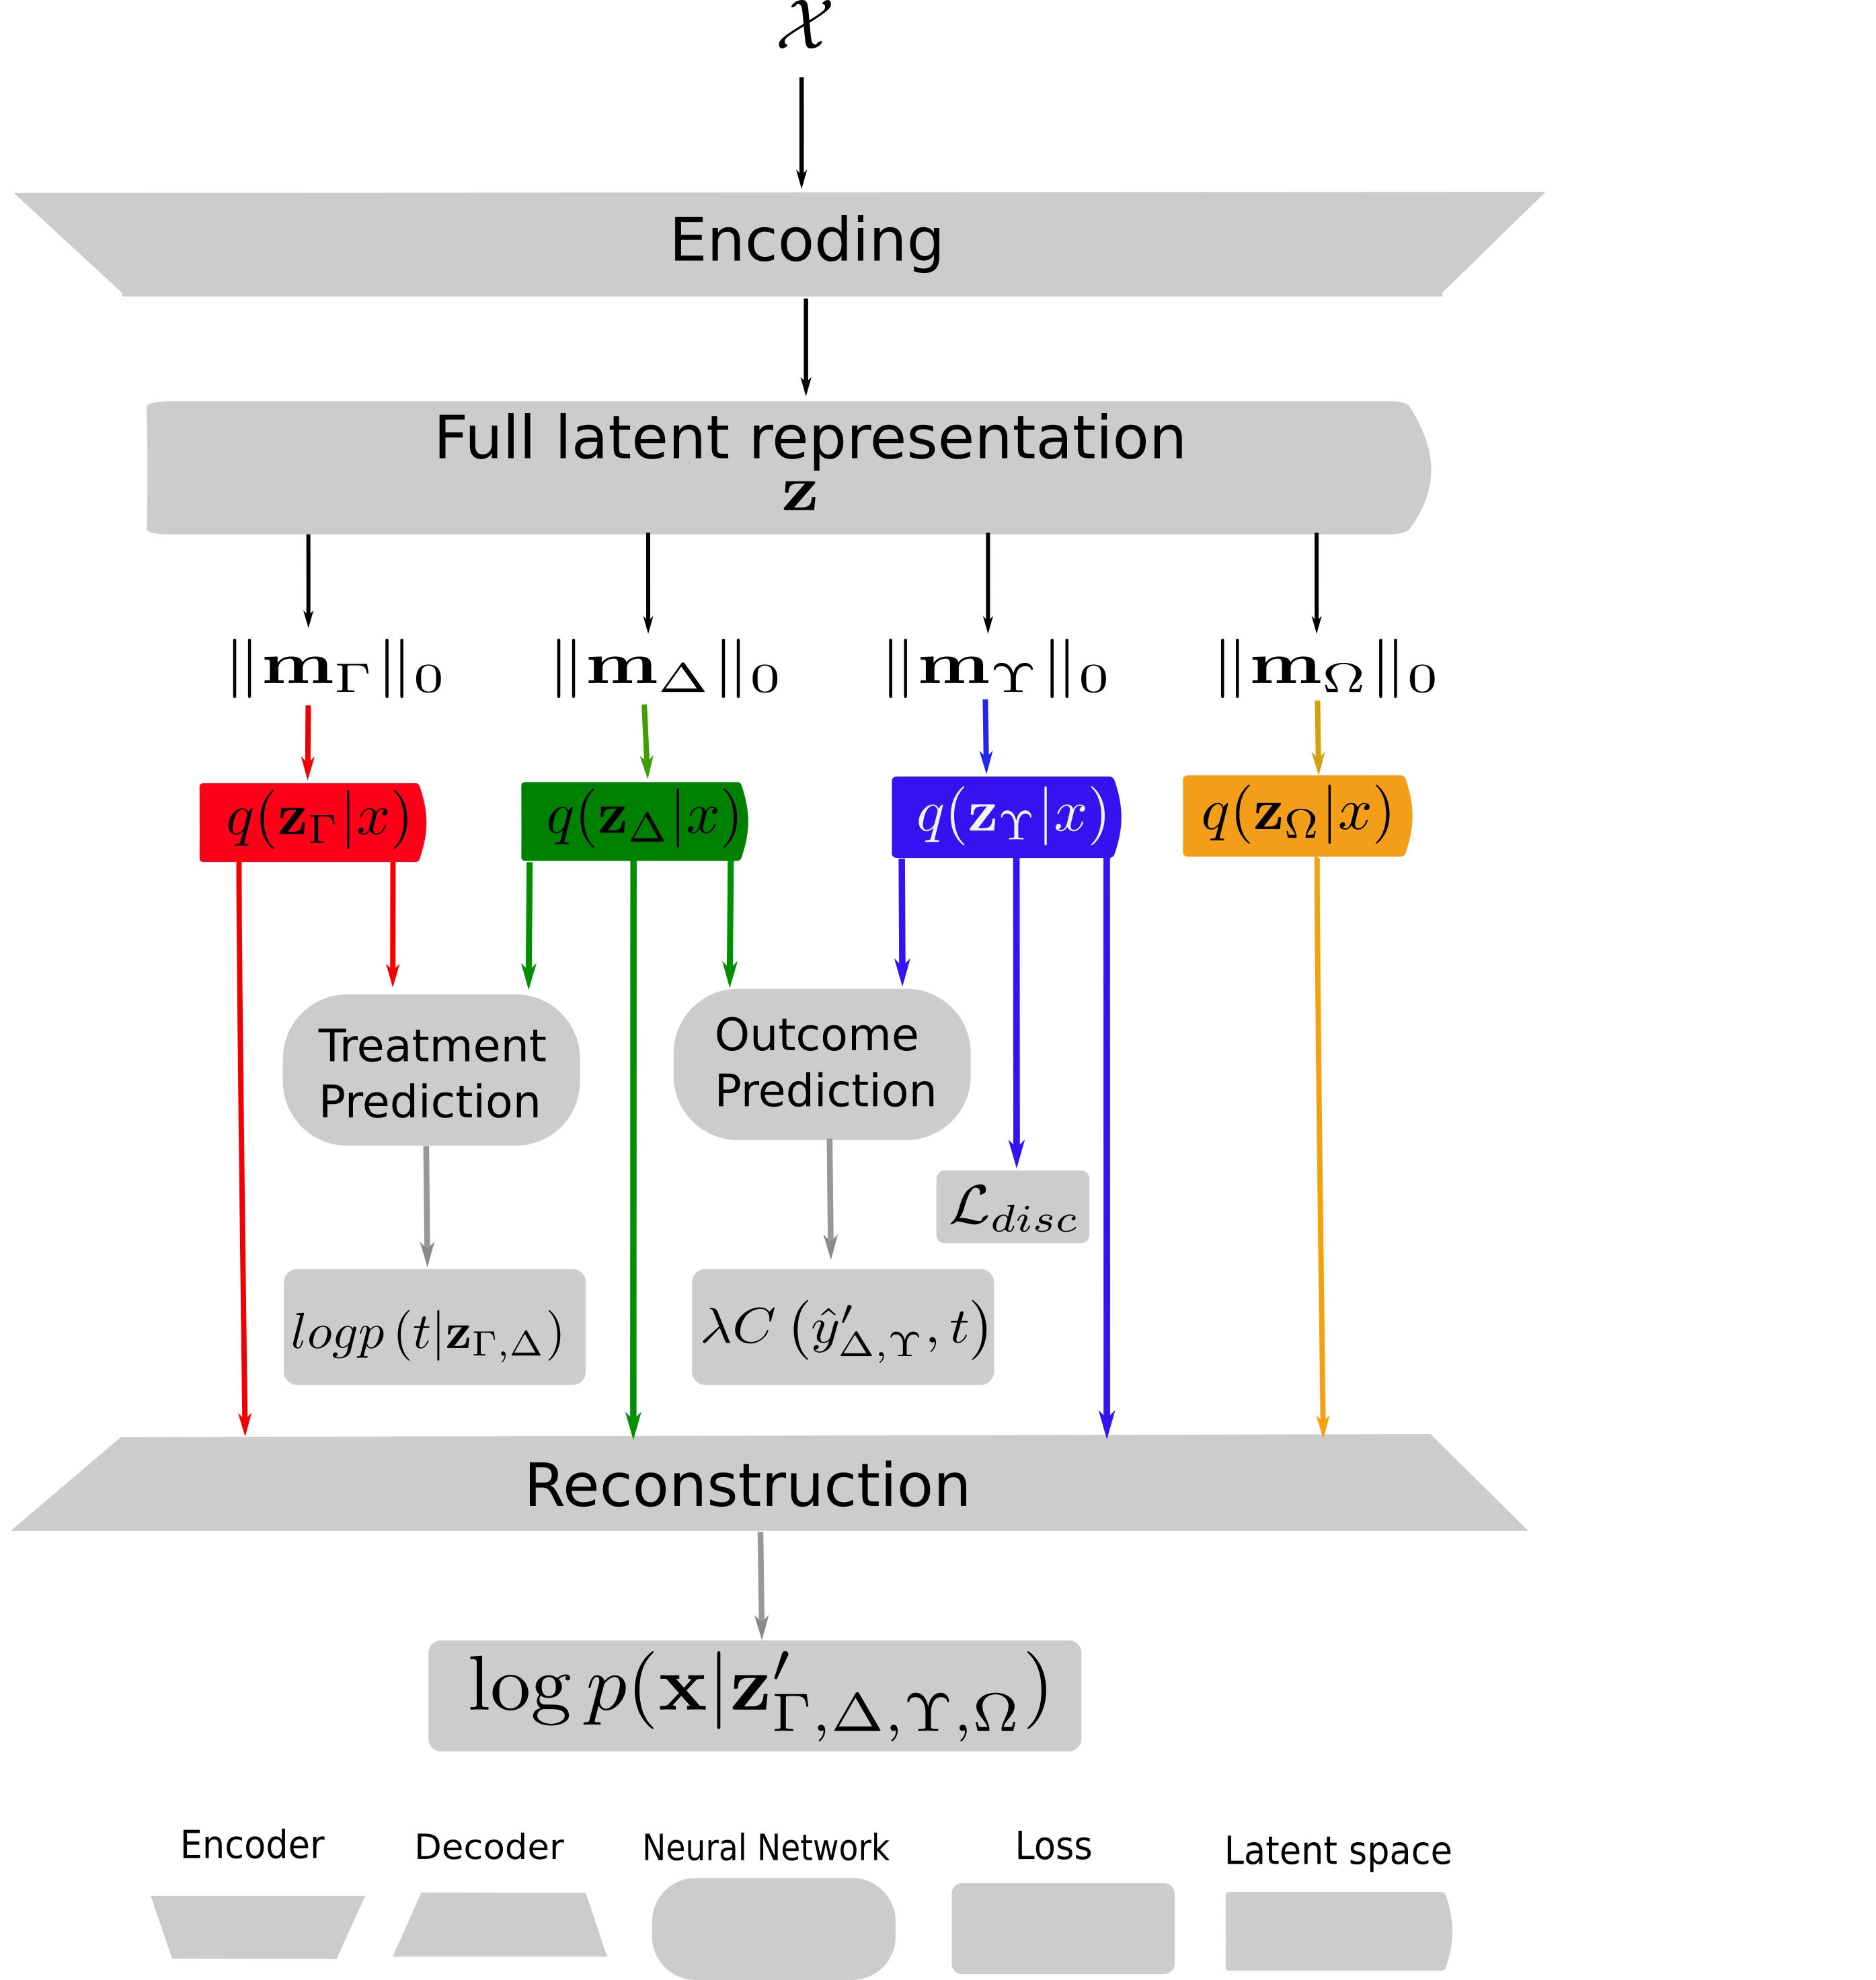
\includegraphics[width=0.45\textwidth]{Images/arch_4.png}
		%\todo[author=jsk]{The routing of the lines could be improved. All lines should enter a block from the top. Perhaps, we can also find a better visual for the masking step. The image also makes no difference between a loss function and the layer / operation that is performed.}
		\caption{Architecture diagram of the GLOVE-ITE (GECO and $L_0$ Optimization for Variational Estimation of Individual Treatment Effects) model: Four embedding spaces are learnt from a shared embedding, each processed through separate masks ($\|\mathbf{m}_{\Gamma}\|_0,\|\mathbf{m}_{\Delta}\|_0,\|\mathbf{m}_{\Upsilon}\|_0,\|\mathbf{m}_{\Omega}\|_0$). These latent spaces serve different roles: $\Gamma$ and $\Delta$ are leveraged for treatment prediction ($\log p( t | \bold{z}_{\Gamma,\Delta}^\prime)$), $\Delta$ and $\Upsilon$ facilitate outcome prediction and constraint enforcement ($C( \hat{y}_{\Delta , \Upsilon}^\prime, t ) $), $\Upsilon$ is used for discrepancy loss ($\mathcal{L}_\mathit{disc}$), $\Omega$ is being used to learn irrelevant variables and all four embeddings jointly contribute to optimizing the reconstruction objective ($\log p( \mathbf{x} | \bold{z}_{\Gamma , \Delta , \Upsilon, \Omega}^\prime  )$).}
		%\todo{Outcome predictor still not shown. The outcome is not a function of the outcome and the constraint is not an output of a regressor. The reconstruction loss is on the masked latent space. Why is the discrepancy loss a function of the reconstruction loss?}
		%\todo{We should show the masking / gating operation in the diagram. It is not clear which task / objective / loss sees the latent space with or without the mask. The lines are not clear. In which direction is the data flowing?}
		%($h^t({y}_{\Delta , \Upsilon}^\prime)$)
		
		
		
		
		\label{fig:arch}
	\end{figure}
	
	\subsection{$L_0$ sparsity objective} 
	\label{sec:l0}
	
	
	%\todo{Work the mask into this. Preferably form the start.}
	
	Our goal is to reduce the causal factors $\mathbf{z}_{\Gamma , \Delta , \Upsilon,\Omega}$ to their true dimensions for the downstream prediction tasks to avoid bias and inclusion of irrelevant factors. For this, we introduce the binary masks $\mathbf{m}_\Gamma$, $\mathbf{m}_\Delta$, $\mathbf{m}_\Upsilon$ and $\mathbf{m}_\Omega$ to define masked version of the latent space, i.e. $\mathbf{z}_\Gamma^\prime = \mathbf{z}_\Gamma \odot \mathbf{m}_\Gamma$, etc. While $L_1$ and $L_2$ regularization objectives are gradient-friendly and lead to small weights, the $L_0$ objective 
	$$
	\| \mathbf {m}\|_0 = \sum_{j=1}^{| \mathbf {m}|} \mathbb{I}[ \mathbf {m}_j \neq 0]
	$$
	induces actual sparsity by counting non-zero elements in the mask. However, $L_0$ is non-differentiable and therefore challenging to optimize.
	
	
	%
	%Regularization adds a term $\mathcal{L}_{reg}$ to the loss function to constrain the weight vector $\boldsymbol{\theta}$, reducing overfitting and improving generalization. In L$_p$ regularization, the penalty is based on the p-norm:
	%
	%\begin{equation}
	%	\mathcal{L}_{\text{reg}} = \|\boldsymbol{\theta}\|_p = \left( |\theta_1|^p + |\theta_2|^p + \cdots \right)^{1/p}
	%\end{equation}
	
	%While L$_1$ and L$_2$ regularizations are gradient-friendly, L$_0$ regularization—counting non-zero elements in 
	%$\boldsymbol{\theta}$—is non-differentiable, making it more challenging to optimize.
	
	This issue can be addressed by shifting to a probabilistic approach where we, instead of the non-zero element count consider the probability of the mask elements being non-zero \citep{louizos2018learning}. For this, we re-define the mask as $\mathbf{m} \sim \text{Bernoulli}( \boldsymbol  \pi)$, where $\boldsymbol{\pi}$ controls the activation probability. The sparsity objective is then the differentiable term $\sum_{j=1}^{| \mathbf{m} |} \boldsymbol  \pi_j$, although the discrete nature of $\mathbf{m}$ still prevents direct gradient-based optimization. 
	\begin{comment}
		For this, we define the mask as $\mathbf{m} = { \mathbf{z}} \odot \mathbf{w} $, where $\mathbf{w} \sim \text{Bernoulli}( \boldsymbol  \pi)$ act as binary gates on a new variable $\tilde{\mathbf{m}}$, and $\boldsymbol{\pi}$ controls the activation probability. The sparsity objective is then the differentiable term $\sum_{j=1}^{| \mathbf{m} |} \boldsymbol  \pi_j$, although the discrete nature of $\mathbf{w}$ still prevents direct gradient-based optimization. 
		content...
	\end{comment}
	
	
	%\todo{I do not understand the role of $\tilde {\mathbf{m}}$. Do we learn it? What is it's value? Is the mask replaced by an expected mask?}
	
	To resolve this, we use the re-parameterization trick and introduce an approximation with a learnable Binary Concrete distribution \citep{maddison2017the}. For this, we sample $\mathbf{u}_i \sim \text{Uniform}(0, 1)$ and introduce another variable
	%
	\begin{equation}
		\mathbf{s}_i 
		= 
		\text{sigmoid}\left(\frac{\beta (\log \mathbf{u}_i - \log (1 - \mathbf{u}_i) + \log \boldsymbol{\alpha}_i)}{\beta}\right),
	\end{equation}
	%
	where parameters $\boldsymbol{\alpha}_i$ and $\beta$ are location and temperature parameters respectively. As $\beta \to 0$, the approximation converges to the original Bernoulli distribution. $\mathbf{m}$ is obtained by stretching the distribution with $\tilde { \mathbf{s}}_i = \mathbf{s}_i (\zeta - \gamma) + \gamma$ using $\gamma < 0$ and $\zeta > 1$. The new sparsity objective is the cumulative distribution function of the learned Binary Concrete distribution, 
	%
	% and applying the hard sigmoid $\mathbf{m}_i = \max \left( 1, \min \left( 0, \tilde{ \mathbf{s}}_i \right) \right)$%
	\begin{equation}
		\begin{aligned}
			%\sum_{j=1}^{|\theta|} (1 - Q(s_j = 0 \mid \alpha, \beta)) =  & \\ 
			\| \mathbf {m}\|_0 
			\approx
			\sum_{j=1}^{| \boldsymbol {m}|} \text{sigmoid} \left(\log \alpha_j - \beta \times \log \left(-\frac{\gamma}{\zeta}\right)\right)
			.
		\end{aligned}
	\end{equation}
	%
	
	%This innovative framework provides a fully differentiable regularization mechanism by combining probabilistic gates with learnable parameters, thus achieving sparsity without compromising the use of gradient-based optimization techniques.
	
	%Combining the VAE objective with this sparsity objective results in Table \ref{tab:IHDP}, as seen in Fig. \ref{fig:learning_curves}. 
	However, combining this sparsity objective with the reconstruction and prediction objectives leads to conflict and it is not trivial to set good constant weights to balance the objectives as seen in Fig. \ref{fig:learning_curves}. Either prediction performance is compromised by restricting the dimensionality to strongly, or unnecessary latent dimensions are included, increasing the risk of bias and predicting outcomes based on irrelevant factors in the downstream task.
	%making explicit trade-off between them necessary. 
	
	\subsection{Prioritizing prediction performance} 
	\label{sec:geco}
	
	During the training of the VAE model, the reconstruction and outcome prediction objectives naturally conflict with the sparsity objective from the previous section. We address this problem by prioritization and only optimize sparsity as long as other tasks perform better than a threshold $\tau$. 
	%
	Generalized ELBO with Constrained Optimization (GECO) \citet{JimenezRezende2018TamingV} achieves this effect for standard VAEs by replacing the reconstruction loss with a constrained expression $C(\dots)$ and introducing a Lagrange multiplier $\lambda$ that is adapted during learning based on the constraint value. We adopt this approach, but replace only the outcome prediction loss:
	\begin{equation}
		\mathcal{L}_{\mathrm{ELBO}} 
		=
		\mathbb{E}_{q(\mathbf{z}_{\Gamma,\Delta,\Upsilon,\Omega} | \mathbf{x})} 
		\Big[ 
		\dots 
		+ 
		\lambda C\left( \hat{y}_{\Delta , \Upsilon}^\prime, t \right)
		\Big] 
		- 
		\mathrm{KL}(\dots)
		\label{eq:elbo-mod}
		,
	\end{equation}
	%
	where the predicted outcome $\hat{y}_{\Delta , \Upsilon}^\prime$ only has access to the masked sections of the latent space $\mathbf{z}_\Delta^\prime$ and $\mathbf{z}_\Upsilon^\prime$.
	%	
	This loss minimizes the KL divergence while enforcing the constraint $\mathbb{E}_{q(\mathbf{z}_{\Gamma,\Delta,\Upsilon,\Omega} | \mathbf{x})} \left[ C\left( \hat{y}_{\Delta , \Upsilon}^\prime, t \right) \right] \leq 0$. We define the constraint expression to enforce an upper bound on the masked outcome prediction task, 
	%
	\begin{equation}
		C\left( \hat{y}_{\Delta , \Upsilon}^\prime, t \right) 
		=  
		\left\| y -  \hat{y}_{\Delta , \Upsilon}^\prime \right \|^2 - \tau
		,
	\end{equation}
	%
	where $y$ is the factual outcome (from the dataset) and predicted from a regressor $h^t({y}_{\Delta , \Upsilon}^\prime)$.
	
	%\todo{I do not understand what the purpose introducing $h$ is. It should predict the outcome and not take it as an input, right? This means thee formula and the figure are both wrong.}
	
	%It ensures the model satisfies the tolerance $\mathbb{E}_{z} \left[ C(x, g(z)) \right] \leq 0$ while optimizing latent representations. 
	%Lagrange multiplier $\lambda \in \mathbb{R}^L
	%$ is used to enforce these constraints, and 
	The modified ELBO form Eq.\ \eqref{eq:elbo-mod} is optimized via a min-max optimization scheme (i.e. dual gradient decent), balancing the objectives and constraints effectively by adjusting $\lambda$ during training. The influence of this constraint and the value of $\lambda$ during training can be observed in Figure \ref{fig:learning_curves}.
	
	%\todo{Is this dual gradient decent?}
	
	%$\left( \mathbf{z}_{\Gamma,\Delta,\Upsilon}, \mathbf{x}, t, y \right)$
	
	%The function $h^t$ predicts the outcomes for both treatments and evaluates the loss based on the predicted outcome corresponding to the observed treatment $t$, utilizing the concatenated latent factors $\Delta$ and $\Upsilon$. The parameter $\tau$ defines a predefined tolerance for outcome prediction.
	
	% It is clear that XXX.
	

\subsection{Mutual Exclusivity Regularization}

To encourage mutual exclusivity across the learned masks, we introduce a softmax-based exclusivity loss that penalizes the sharing of the same latent dimension among different masks. Let $\mathcal{M} \in \mathbb{R}^{4 \times d}$ denote the stacked mask logits for the four masks, where $d$ is the latent dimensionality. We compute a temperature-controlled softmax across the rows of $\mathcal{M}$ to obtain the normalized mask assignments:
\begin{equation}
	\mathbf{S} = \text{softmax}\left(\frac{\mathcal{M}}{\kappa}\right),
\end{equation}
where $\kappa > 0$ is the temperature parameter controlling the sharpness of the assignments. The exclusivity loss is then defined as the mean column-wise entropy of $\mathbf{S}$:
\begin{equation}
	\mathcal{L}_{\text{excl}} = -\frac{1}{d} \sum_{j=1}^d \sum_{i=1}^4 S_{i,j} \log S_{i,j}.
\end{equation}
Minimizing $\mathcal{L}_{\text{excl}}$ encourages each latent dimension to be assigned predominantly to a single mask, thereby reducing redundancy and promoting specialization across the latent representations.

	
	\subsection{Implementation Details}
	\label{sec:details}
	%\todo{Notation hell!!!}
	
	The overall loss function of our approach consists of the $L_0$ sparsity objective on masks $\mathbf{m}_{\Gamma}$,  $\mathbf{m}_{\Delta}$, $\mathbf{m}_{\Upsilon}$ and $\mathbf{m}_{\Omega}$ from Section \ref{sec:l0}, the modified ELBO with the outcome prediction constraint from Section \ref{sec:geco}, and a discrepancy loss on the latent space between the treatment groups $\mathcal{L}_\mathit{disc}$, 
	%
	\begin{equation}
		\mathcal{L}_\mathit{GLOVE-ITE}=\mathcal{L}_{\text{ELBO}} + \|\mathbf{m}_{\Gamma, \Delta, \Upsilon,\Omega}\|_0 + \mathcal{L}_{\mathit{excl}}+\mathcal{L}_\mathit{disc}
		\label{eq:overall}
		.
	\end{equation}
	%
	With all terms, the modified ELBO has the following form,
	%
	\begin{equation}
		\begin{aligned}
			\mathcal{L}_{\text{ELBO}} 
			= 
			& 
			\mathbb{E}_{q(\mathbf{z}_{\Gamma,\Delta,\Upsilon,\Omega} | \mathbf{x})} 
			\Big[
			\log p\left( \mathbf{x} | \bold{z}_{\Gamma , \Delta , \Upsilon,\Omega}^\prime  \right)
			+ 
			\log p\left( t | \bold{z}_{\Gamma,\Delta}^\prime \right)\\
			&
			+
			\lambda C\left(\hat{y}_{\Delta , \Upsilon}^\prime, t \right)
			\Big]
			- 
			\mathrm{KL}(q(\bold{z}_{\Gamma,\Delta, \Upsilon,\Omega}^\prime   | \mathbf{x}) \parallel p(\bold{z}_{\Gamma,\Delta, \Upsilon,\Omega}))
		\end{aligned}  
		\label{eq:elbo-mod}
	\end{equation}
	%
	\begin{comment}
		Not that both, outcome prediction and treatment prediction, are based on the masked latent spaces, while the reconstruction loss sees the unmasked latent space.
		\todo{Check that this is correct!!!}
		content...
	\end{comment}
	
	
	%
	%
	%where the term $\log p\left({x}|\bold{z}_{\Gamma , \Delta , \Upsilon}\right)$ represents the reconstruction loss (Mean Squared Error:MSE), which measures how well $x$ can be reconstructed from the representations of the three latent factors. This loss serves to ensure the quality of both the encoding and the disentanglement of the learned latent representations. While, $\log p\left({t}|\bold{z}_{\Gamma,\Delta} \right)$ represents the classification loss, modeled using Binary Cross-Entropy (BCE). This component facilitates learning of the $\Gamma$ and $\Delta$ embeddings by predicting the treatment assignment $t$ , thereby guiding the optimization of these two latent factors.
	%
	%Let $\boldsymbol{m}$ denote the learned mask of the embedding, such that $\boldsymbol{z}_{\Delta} = \left( \boldsymbol{z} \odot \boldsymbol{m}_{\Delta} \right)$. Consequently, both reconstruction and classification losses can be expressed as implicit vector products with the masks, in general can be formulated as:
	
	%\begin{equation}
	%	 \log p\left({k}|\bold{z}_{\Gamma,\Upsilon} \right)=  \log p(k |\Gamma \odot\boldsymbol{m}_{\Gamma} , \Upsilon \odot\boldsymbol{m}_{\Upsilon} ).
	%\end{equation}
	
	%The $\lambda C\left({y}_{\Delta , \Upsilon},t \right)$ is constrained regression loss for the prediction of the outcome, elaborated in Section \ref{sec:geco}
	
	
	%${\text{KL}}$ represents the Kullback-Leibler divergence between approximated posterior $q(\mathbf{z}|\mathbf{x})$ and prior $p(\mathbf{z})$ of respective latent factor. 
	
	%$\|\boldsymbol{m}_{\Gamma, \Delta, \Upsilon }\|_0$ term enforces sparsity within the latent representations of each factor. It learns the mask that explicitly determines which latent dimensions to retain and which to set to zero, ensuring sparsity while adhering to the predefined outcome constraint, explained in Section \ref{sec:l0}.
	\begin{comment}
		\begin{equation}
			\|\mathcal{M}_{v}\|_0=\sum_{j=1}^{|\mathcal{M}_{v}|} \text{sigmoid} \left(\log \alpha_j - \beta \times \log \left(-\frac{\gamma}{\zeta}\right)\right),
		\end{equation}
		where $\alpha$ serves as the location parameter, while $\beta$ (temperature)  controls the smoothness of the approximation. The constraints $\gamma < 0$, $\zeta > 1 $ ensure the mask values remain within the $(0,1)$ interval. Further details are provided in Section \ref{l0}.
	\end{comment}
	
	
	Finally, the discrepancy loss is defined between the masked distribution of the $\Upsilon$-section of the latent space for the two different treatment cases $\mathbf{Z}_{\Upsilon}^\prime | t=0$ and $\mathbf{Z}_{\Upsilon}^\prime | t=1$
	%
	\begin{eqnarray}
		\mathcal{L}_{disc}
		=
		wass
		[\mathbf{Z}_{\Upsilon}^\prime | t=0,
		\mathbf{Z}_{\Upsilon}^\prime | t=1],
	\end{eqnarray}
	%
	\textbf{{$\mathcal{L}_{disc}$}} ensures that $\Upsilon$ remains independent of $\Gamma$, effectively reducing the influence of 
	$\Gamma$ on $\Upsilon$. This mitigates selection bias introduced by $\Gamma$, enabling unbiased predictions for the downstream task. To achieve this, we employ the Wasserstein distance as the discrepancy loss as proposed by \citep{Khan2024OnTE}.
	
	\section{Experiments}
	In this section, we present the evaluation criteria for treatment effect estimation, describe the datasets utilized in our experiments, experiment details, results and conclude with a qualitative analysis of the proposed method. 
	\subsection{Evaluation criteria}
	A widely used metric for evaluating treatment effect estimation is the Precision in Estimation of Heterogeneous Effect (PEHE), defined as:
	\begin{equation}
		\mathit{PEHE}=\sqrt{\frac{1}{N}\sum_{i=1}^{N}(\hat{e}_{i}-e_{i})^2}
	\end{equation}
	where $\hat{e}_{i}=\hat{y}_{i}^{1}-\hat{y}_{i}^{0}$ represents the predicted effect, and ${e}_{i}={y}_{i}^{1}-{y}_{i}^{0}$ denotes the true effect.
	
	\begin{table*}[!ht]
		\centering
		\caption{PEHE (std) results (lower is better) on the IHDP dataset (first 30 realizations), evaluated across varying number of irrelevant variables ($\#\Omega$) and the active latent dimensionality used by each encoder during learning.}
		\begin{tabular}{lrrrrrrr}
			\toprule
			Method & $\#\Omega$ & $\Gamma$-active & $\Delta$-active & $\Upsilon$-active & $\Omega$-active & Total-active & PEHE \\
			\midrule
			
			DR-CFR		&5	& 35 & 35      & 35           & NA   & 105          & 	1.09 (0.51)							\\
			%RLO-DRCFR	&5 & 35 & 35      & 35           & NA   & 105          & 	1.09 (0.51)							\\
			TEDVAE    	& 5          	& 35 & 35      & 35           & NA   & 105          & 0.88 (0.62)           \\
			TVAE   		& 5     		& 35 & 35      & 35           & 35   & 140          & 0.87 (0.47)        \\
			DRI-ITE     & 5         	& 35 & 35      & 35           & 35   & 140          & 1.09 (0.53)           \\
			GLOVE-ITE (Ours)    	& 5           	& 7 & 9      & 9           & 7   & 32          & \textbf{0.70 (0.07)}          \\
			
			\bottomrule
			DR-CFR		&5	& 35 & 35      & 35           & NA   & 105          & 		1.15 (0.61)						\\
			%RLO-DRCFR	&5 & 35 & 35      & 35           & NA   & 105          & 			1.15 (0.62)						\\
			TEDVAE    	& 10          	& 35 & 35      & 35           & NA   & 105          & 1.11 (0.80)           \\
			TVAE   		& 10       	& 35 & 35      & 35           & 35   & 140          & 1.10 (0.49)        \\
			DRI-ITE     & 10        	& 35 & 35      & 35           & 35   & 140          & 1.15 (0.51)           \\
			GLOVE-ITE (Ours)    	& 10           & 7 & 9      & 9           &   8 & 33          & \textbf{0.74 (0.08)}          \\
			
			\bottomrule
			DR-CFR		&5	& 35 & 35      & 35           & NA   & 105          & 		1.19 (0.58)						\\
			%RLO-DRCFR	&5 & 35 & 35      & 35           & NA   & 105          & 			1.18 (0.59)					\\
			TEDVAE    	& 15          	& 35 & 35      & 35           & NA   & 105          & 1.27 (0.87)           \\
			TVAE   		& 15      	& 35 & 35      & 35           & 35   & 140          & 1.23 (0.52)        \\
			DRI-ITE     & 15         	& 35 & 35      & 35           & 35   & 140          & 1.18 (0.58)           \\
			GLOVE-ITE (Ours)    	& 15           & 7 & 8      & 8           & 7   & 30          & \textbf{0.75 (0.08)}         \\
			
			
			\bottomrule
		\end{tabular}
		
		\label{tab:IHDP}
		
	\end{table*}
	\subsection{Datasets}
	We evaluate our approach using both real-world and synthetic datasets. Synthetic data enables qualitative analysis of the model while assessing its performance in treatment effect estimation.
	\begin{itemize}
		
		\item \textbf{Infant Health and Development Program (IHDP)}: The IHDP dataset, derived from an RCT by \citet{Gunn} and adapted by \citet{Hill} to introduce selection bias, contains 25 covariates describing child and mother characteristics. It includes 747 instances (139 treated, 608 control) and evaluates the effect of specialist home visits on children’s cognitive health. Since IHDP lacks irrelevant variables, we augment it with artificial contrasts for evaluation \citep{Khan2024OnTE}.
		
		\item \textbf{Synthetic}: We use the same settings of syntehtic datasets as used by \citet{Negar,Khan2024OnTE}, generated with a sample size 
		$N$, dimensions $\left[{d}_{\Gamma},{d}_{\Delta},{d}_{\Upsilon},{d}_{\Omega}\right]$, and specified mean and covariance matrices ($\mu_{L},\sum_{L}$) for each latent factor $L \in \left[\Gamma,\Delta,\Upsilon,\Omega \right]$. Data is sampled from a multivariate normal distribution, forming a covariate matrix of size $N \times (d_{\Gamma}+d_{\Delta}+d_{\Upsilon}+{d}_{\Omega})$. Irrelevant variables are added by permuting values from other factors to ensure realistic complexity.
		
		
	\end{itemize}
	\begin{table*} [!ht]
		\centering
		\caption{PEHE (std) results (lower is better) on the synthetic dataset (8×8×8×$\Omega$), evaluated across varying number of irrelevant variables ($\#\Omega$) and the active latent dimensionality used by each encoder during learning.}
		\begin{tabular}{lrrrrrrr}
			\toprule
			Method & $\#\Omega$  & $\Gamma$-active & $\Delta$-active & $\Upsilon$-active & $\Omega$-active & Total-active & PEHE  \\
			\midrule
			DR-CFR		&5				& 30 & 30      & 30           & NA   & 90      		&0.23 (0.001)	\\
			%RLO-DRCFR	& 5				& 30 & 30      & 30           & NA   & 90     		&0.26 (0.009)	\\
			TEDVAE    	& 5          	& 30 & 30      & 30           & NA   & 90          	& 0.22 (0.012)           \\
			TVAE   		& 5      		& 30 & 30      & 30           & 30   & 120          & 0.23 (0.003)        \\
			DRI-ITE     & 5       		& 30 & 30      & 30           & 30   & 120          & 0.26 (0.024)           \\
			GLOVE-ITE (Ours)   	& 5          	& 9 & 11      & 7           & 5   & 32      & \textbf{0.17 (0.007)}          \\
			
			\bottomrule
			DR-CFR		&10	& 30 & 30      & 30           & NA   & 90      & 0.27 (0.016)		\\
			%RLO-DRCFR	& 10	& 30 & 30      & 30           & NA   & 90      &0.28 (0.003)	\\
			TEDVAE    	& 10         	& 30 & 30      & 30           & NA   & 90          & 0.50 (0.054)           \\
			TVAE   		& 10       		& 30 & 30      & 30           & 30   & 120          & 0.28 (0.004)        \\
			DRI-ITE     & 10      		& 30 & 30      & 30           & 30   & 120          & 0.27 (0.027)           \\
			GLOVE-ITE (Ours)    	& 10           	& 8 & 11      & 7           &3   & 29          & \textbf{0.18 (0.004)}          \\
			
			\bottomrule
			DR-CFR		&15	& 30 & 30      & 30           & NA   & 90      &0.28 (0.019)	\\
			%RLO-DRCFR	&15	& 30 & 30      & 30           & NA   & 90      &0.32 (0.046)	\\
			TEDVAE    	& 15        	& 30 & 30      & 30           & NA   & 90          & 0.49 (0.010)           \\
			TVAE   		& 15      		& 30 & 30      & 30           & 30   & 120          & 0.34 (0.003)        \\
			DRI-ITE     & 15       		& 30 & 30      & 30           & 30   & 120          & 0.28 (0.021)           \\
			GLOVE-ITE (Ours)    	& 15           	& 8 & 10      & 6           & 2   & 26          & \textbf{0.17 (0.004)}          \\
			
			\bottomrule
		\end{tabular}
		
		\label{tab:synthetic}
		%\todo{Refer to the bottleneck size as $m_{\Gamma}$ as introduced in the method section.}
	\end{table*}
	
	\begin{figure*}[!ht]
		\centering
		%\captionsetup{justification=centering}
		
		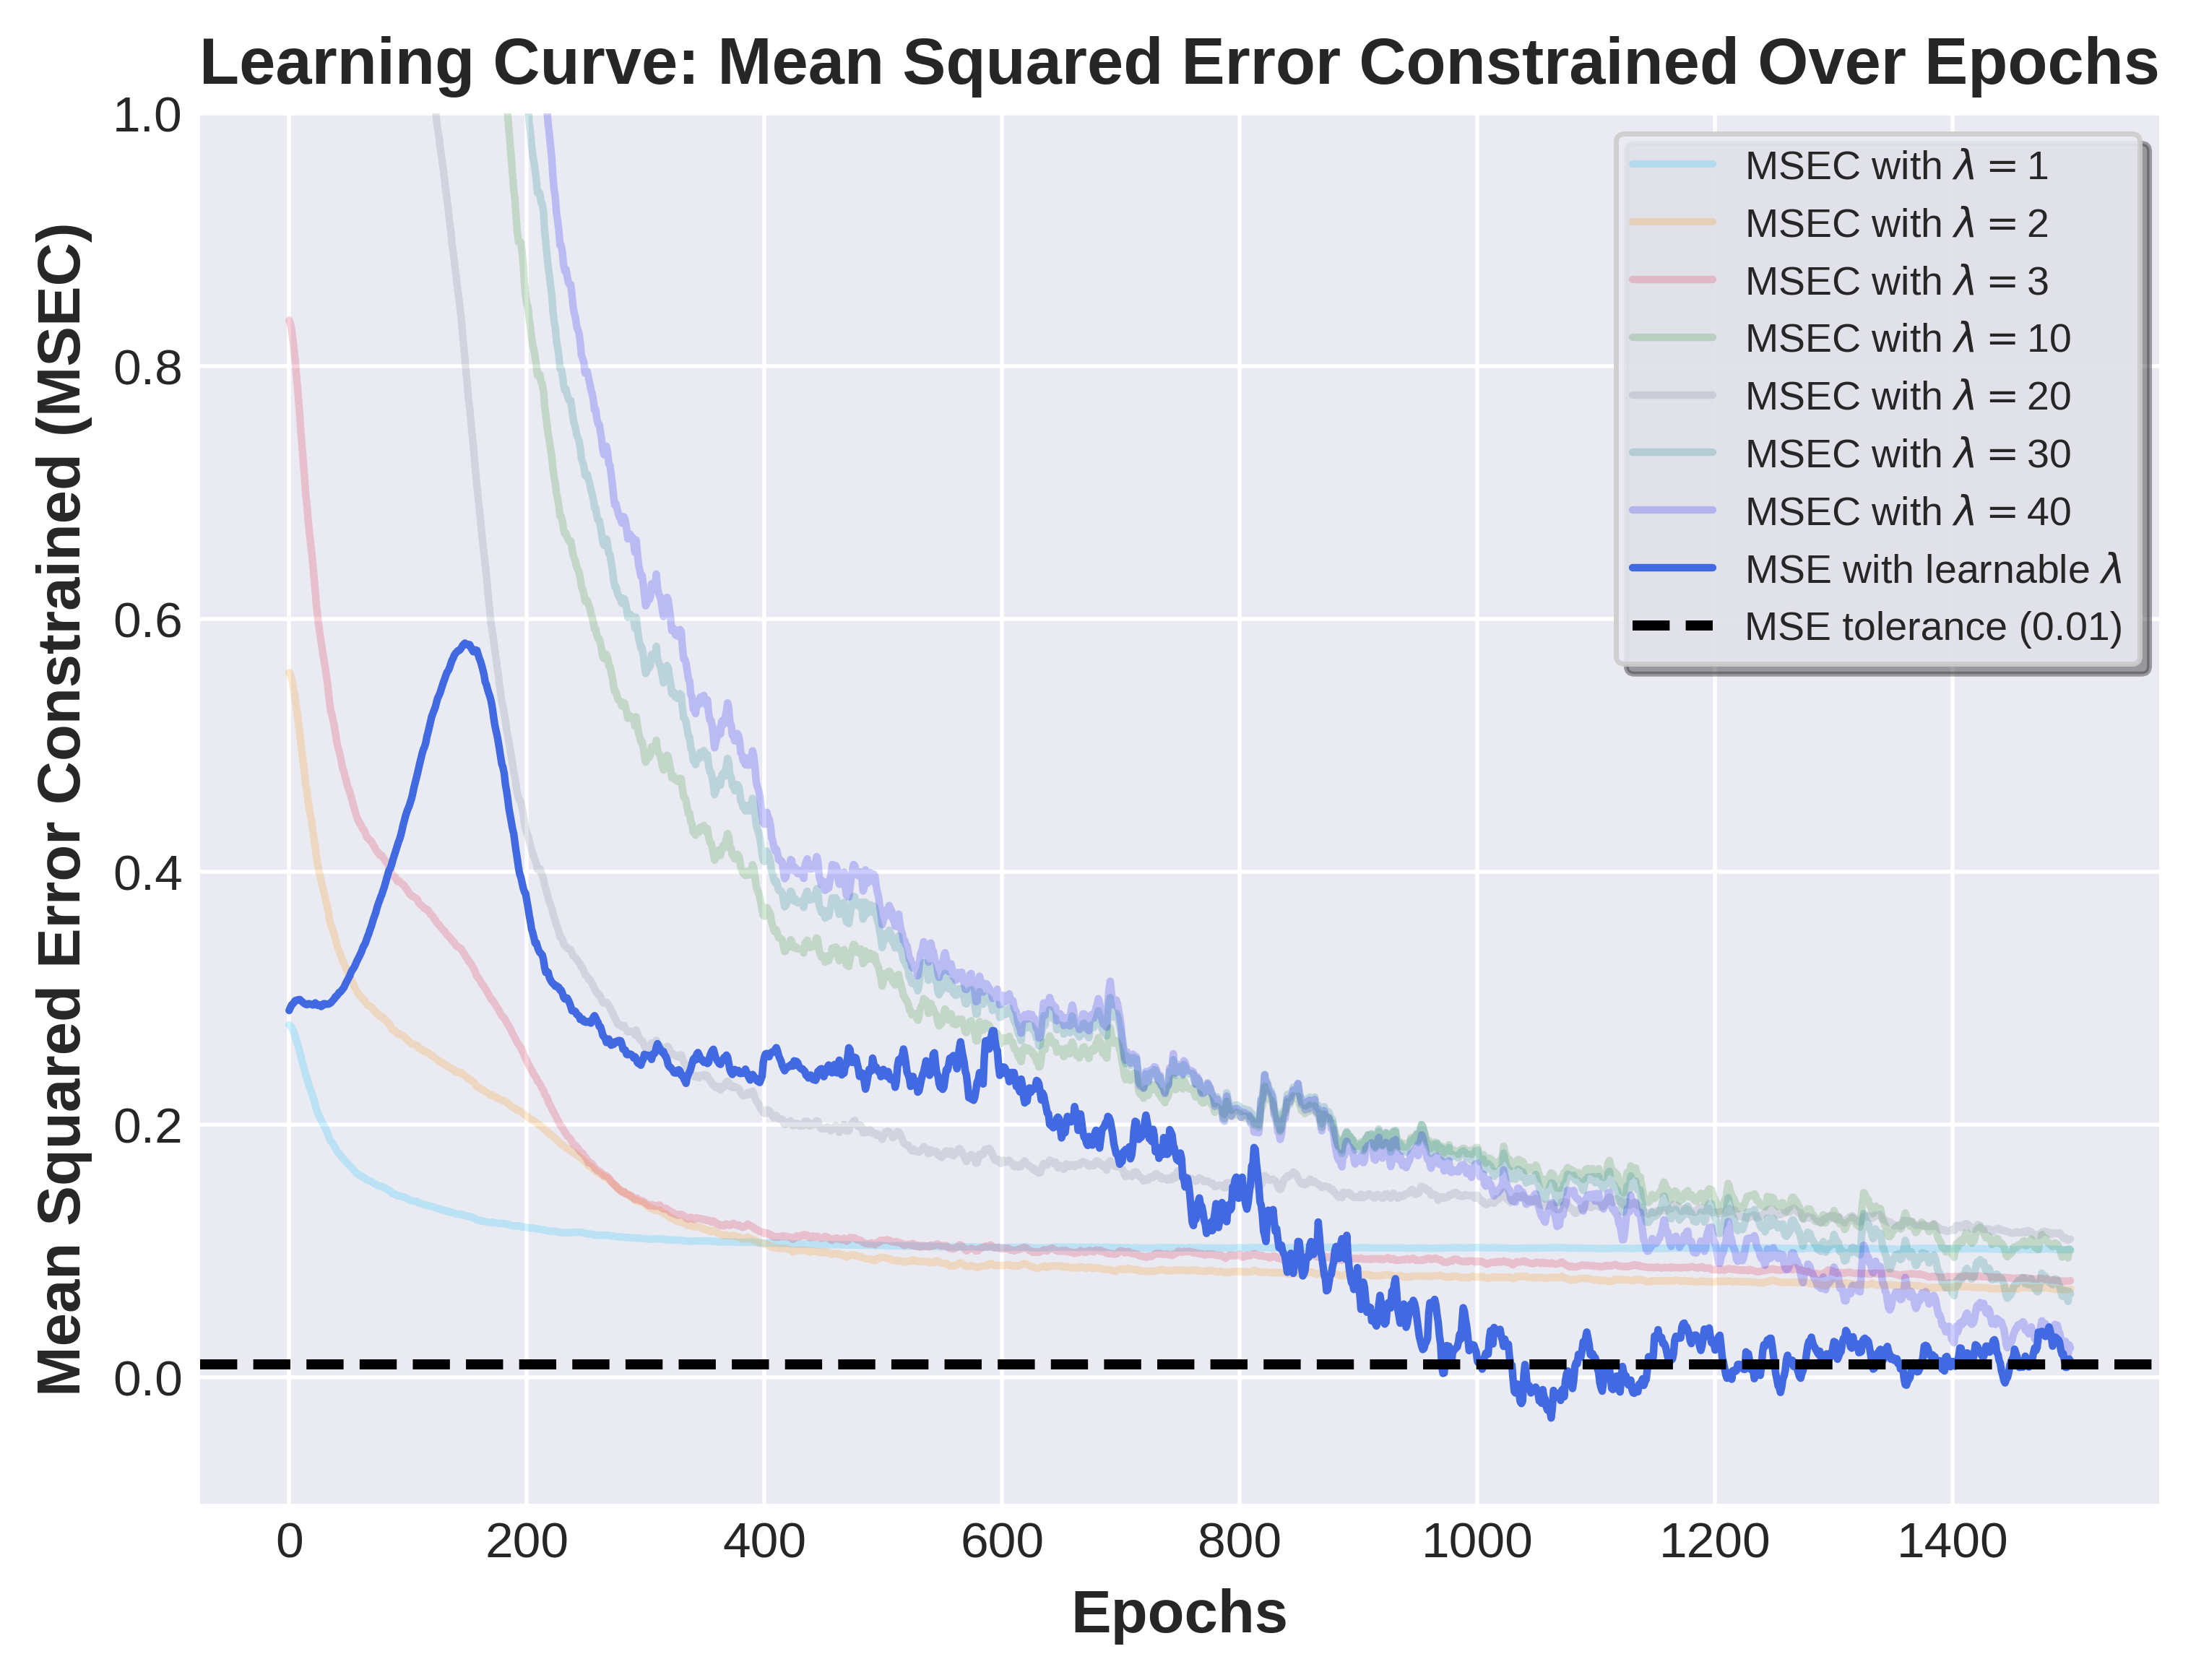
\includegraphics[width=0.33\textwidth]{Images/MSE_wo_GECO.png}
		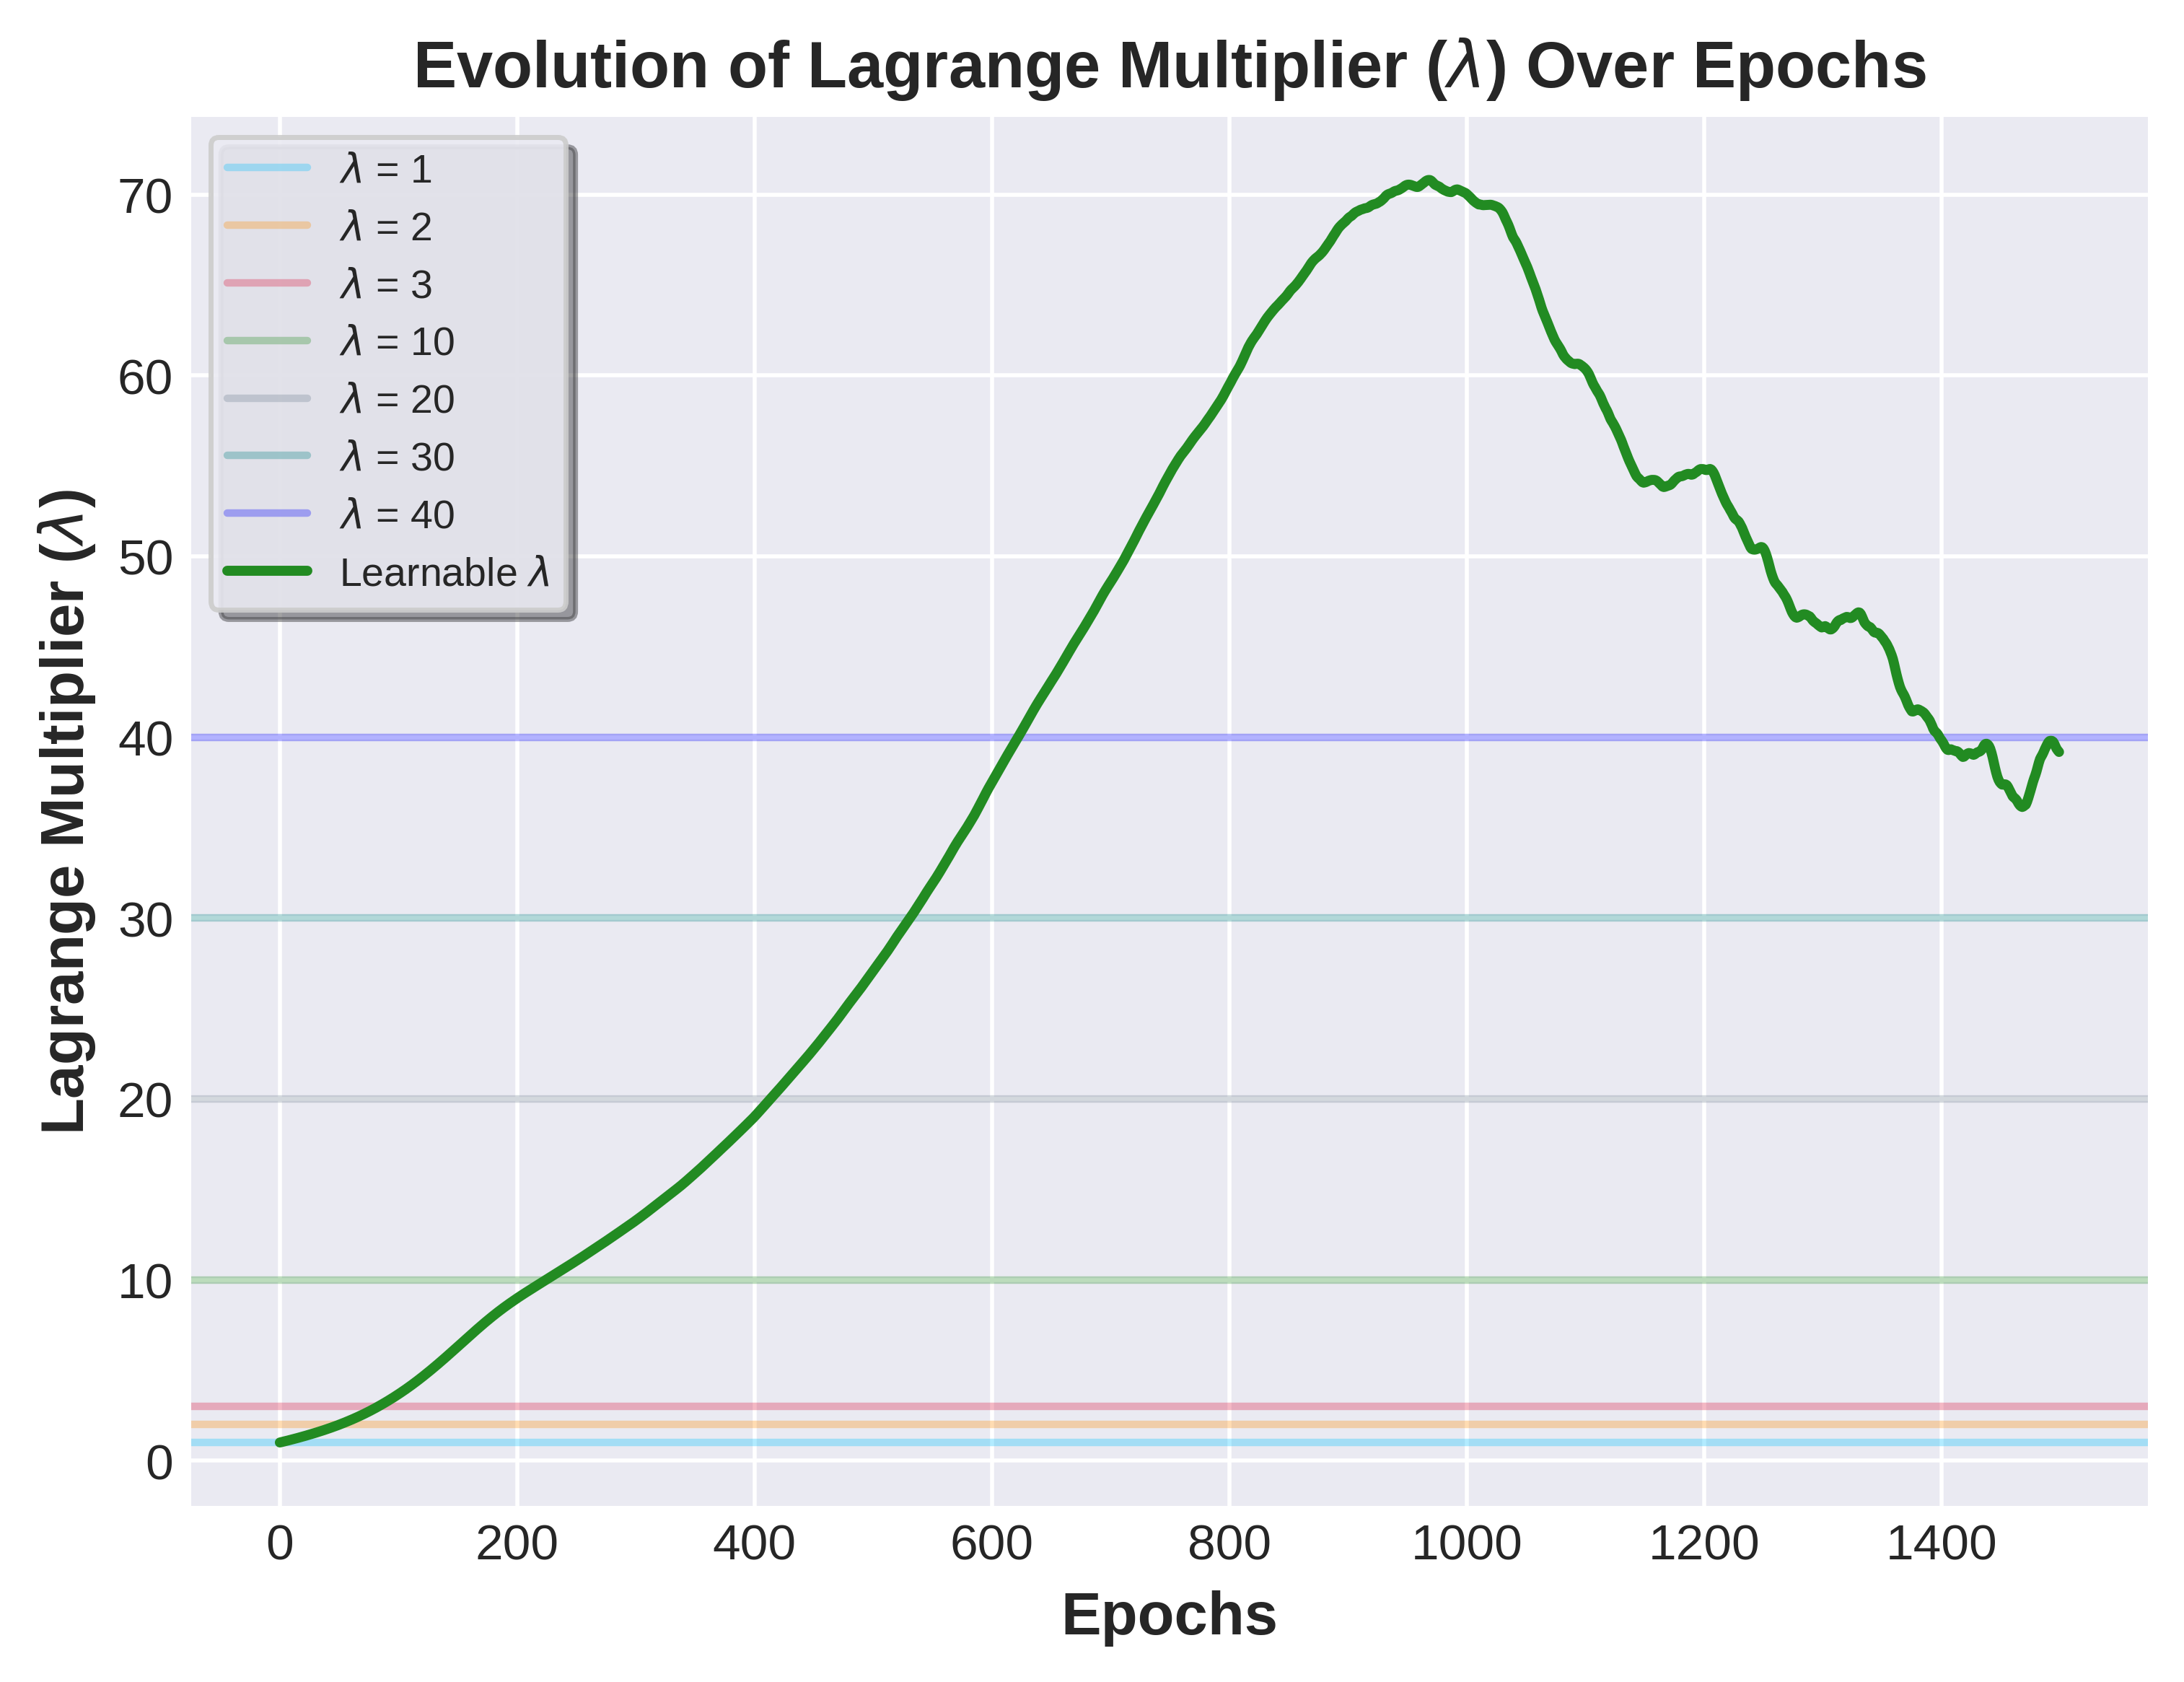
\includegraphics[width=0.33\textwidth]{Images/langragian_multiplier_wo_GECO.png}
		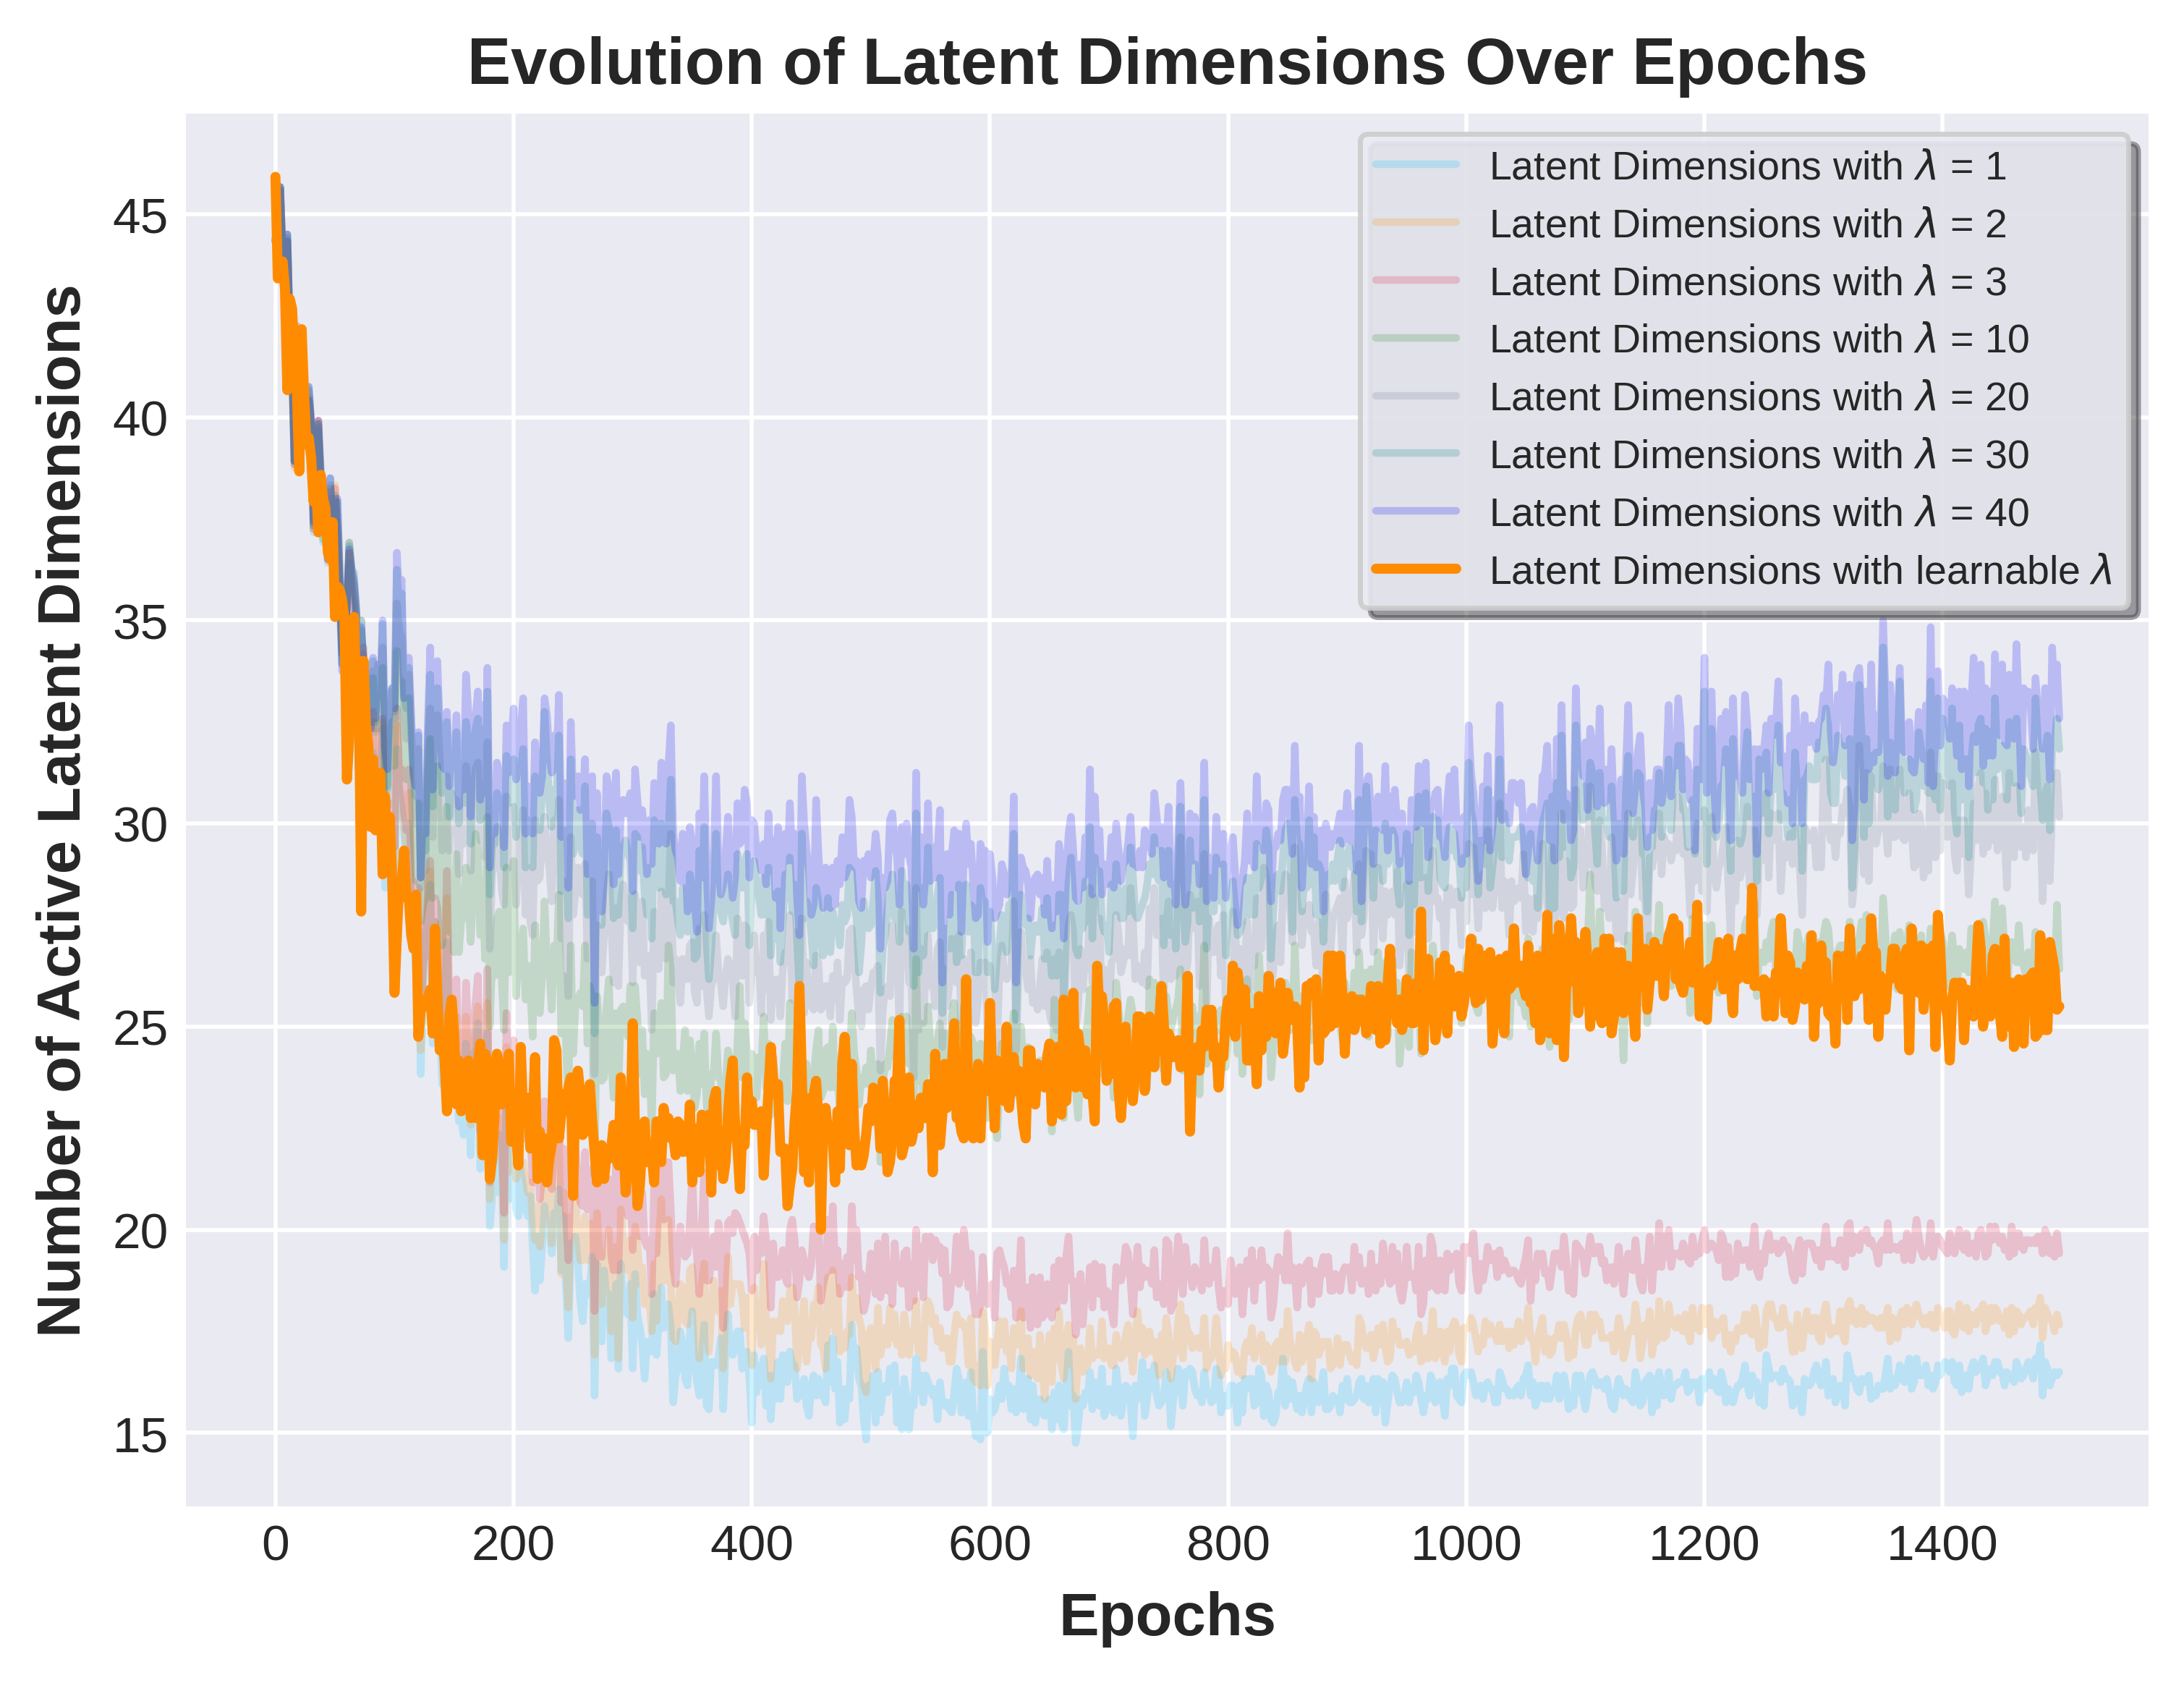
\includegraphics[width=0.33\textwidth]{Images/latent_dims_wo_GECO.png}
		
		\caption{Visualization of three key training metrics: Mean Squared Error Constrained (MSEC:can be negative) relative to the threshold $\tau$, the Lagrange multiplier ($\lambda$), and the number of active latent dimensions on synthetic data with an 8×8×8 dimensional structure. Dimmed lines represent fixed $\lambda$, while brighter lines indicate learnable $\lambda$ (best viewed in color).}
		
		\label{fig:learning_curves}
		%\todo{Intermediate lines and 2D pareto plot still missing.}	
		%\todo{What dataset? What number of irrelevant dimensions (ground truth)?}	
	\end{figure*}
	
	
	\subsection{Experiment details}
	\textbf{IHDP Dataset:}
	We utilized a single representational network with three layers and an input of $40$ dimensions. The hidden and output layers contained $100$ and $40$ neurons respectively. The network was trained using the Adam optimizer with ELU activation, a batch size of $500$, and a learning rate of $1{e}{-5}$ over a maximum of $8000$ epochs. The best model was selected using PEHE on the validation set, following the approach in \citet{UriSha}. Data splitting for training, validation, and testing matched the protocol with $20$\% of the training data reserved for validation. For GECO, we set $\lambda_{min}=0$, 
	$\lambda_{max}=200$, $\lambda_{init}=1$, $\alpha=0.99$, and an MSE tolerance ($\tau$) of 0.4. For $L_0$ regularization, we used $beta=0.6$, $\gamma=-0.1$, and $\zeta=1.1$
	%in \citet{UriSha,Negar},
	\textbf{Synthetic Dataset:}
	The same settings were applied with the following modifications: input and output dimensions for the encoder were $60$, batch size was $512$, maximum epochs were limited to $1500$, and MSE tolerance was set to $0.01$.
	
	
	\subsection{Results}
	
	The Table \ref{tab:IHDP} presents a comprehensive evaluation of treatment effect estimation methods on the IHDP dataset, highlighting the superior performance of our approach across varying dimensions of irrelevant variables ($\Omega$). GLOVE-ITE consistently achieves the lowest Precision in Estimation of Heterogeneous Effect (PEHE) values: 0.75(0.39), 0.75(0.38), and 0.78(0.41) for $\Omega$=5,10,15 respectively; outperforming strong baselines such as TEDVAE, TVAE, and DRI-ITE. Notably, GLOVE-ITE achieves this accuracy with significantly reduced total dimensionality (e.g., 39 vs. 140 for $\Omega$=5), showcasing its ability to narrow down the VAE bottleneck and discarding unnecessary latent dimensions. Furthermore, GLOVE-ITE demonstrates remarkable robustness to increasing irrelevant dimensions, exhibiting minimal degradation in PEHE compared to other methods. In contrast, baselines either rely on higher dimensional representations or exhibit inferior accuracy, underscoring the efficiency and effectiveness of our approach in solving complex treatment effect estimation tasks.
	
	
	
	\begin{comment}
		\begin{figure*}
			\centering
			%\captionsetup{justification=centering}
			
			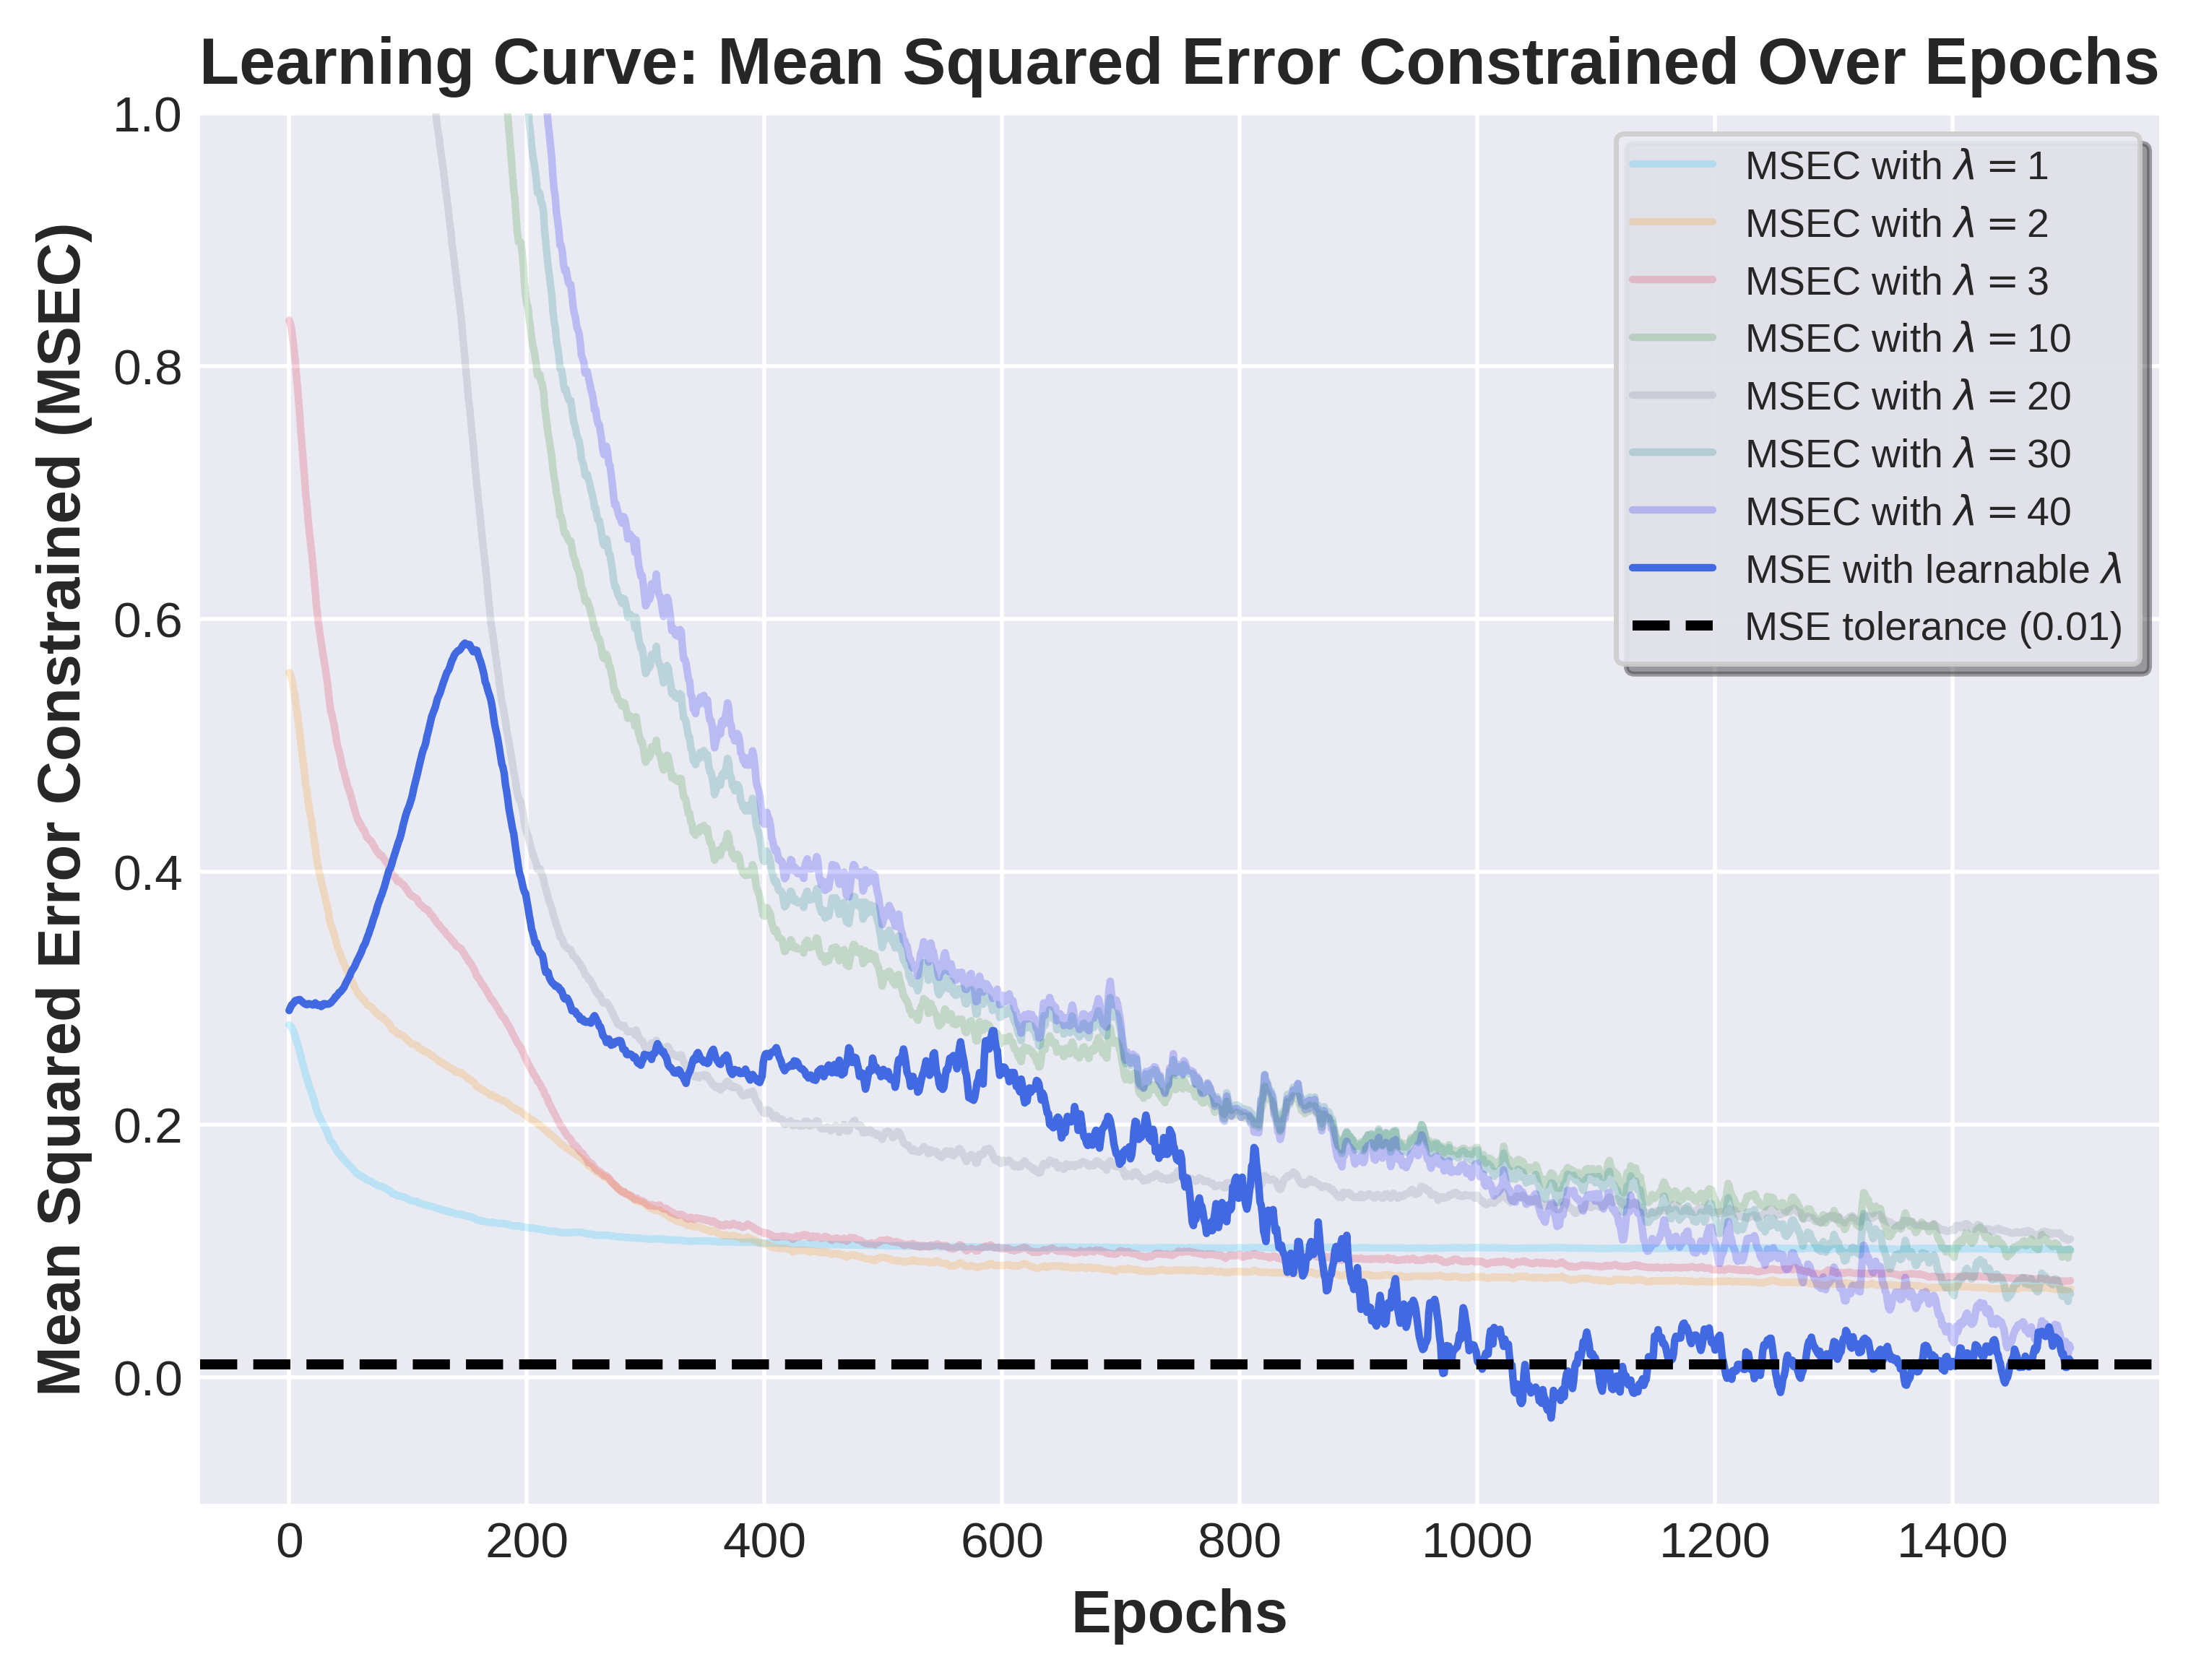
\includegraphics[width=0.32\textwidth]{Images/MSE_wo_GECO.png}
			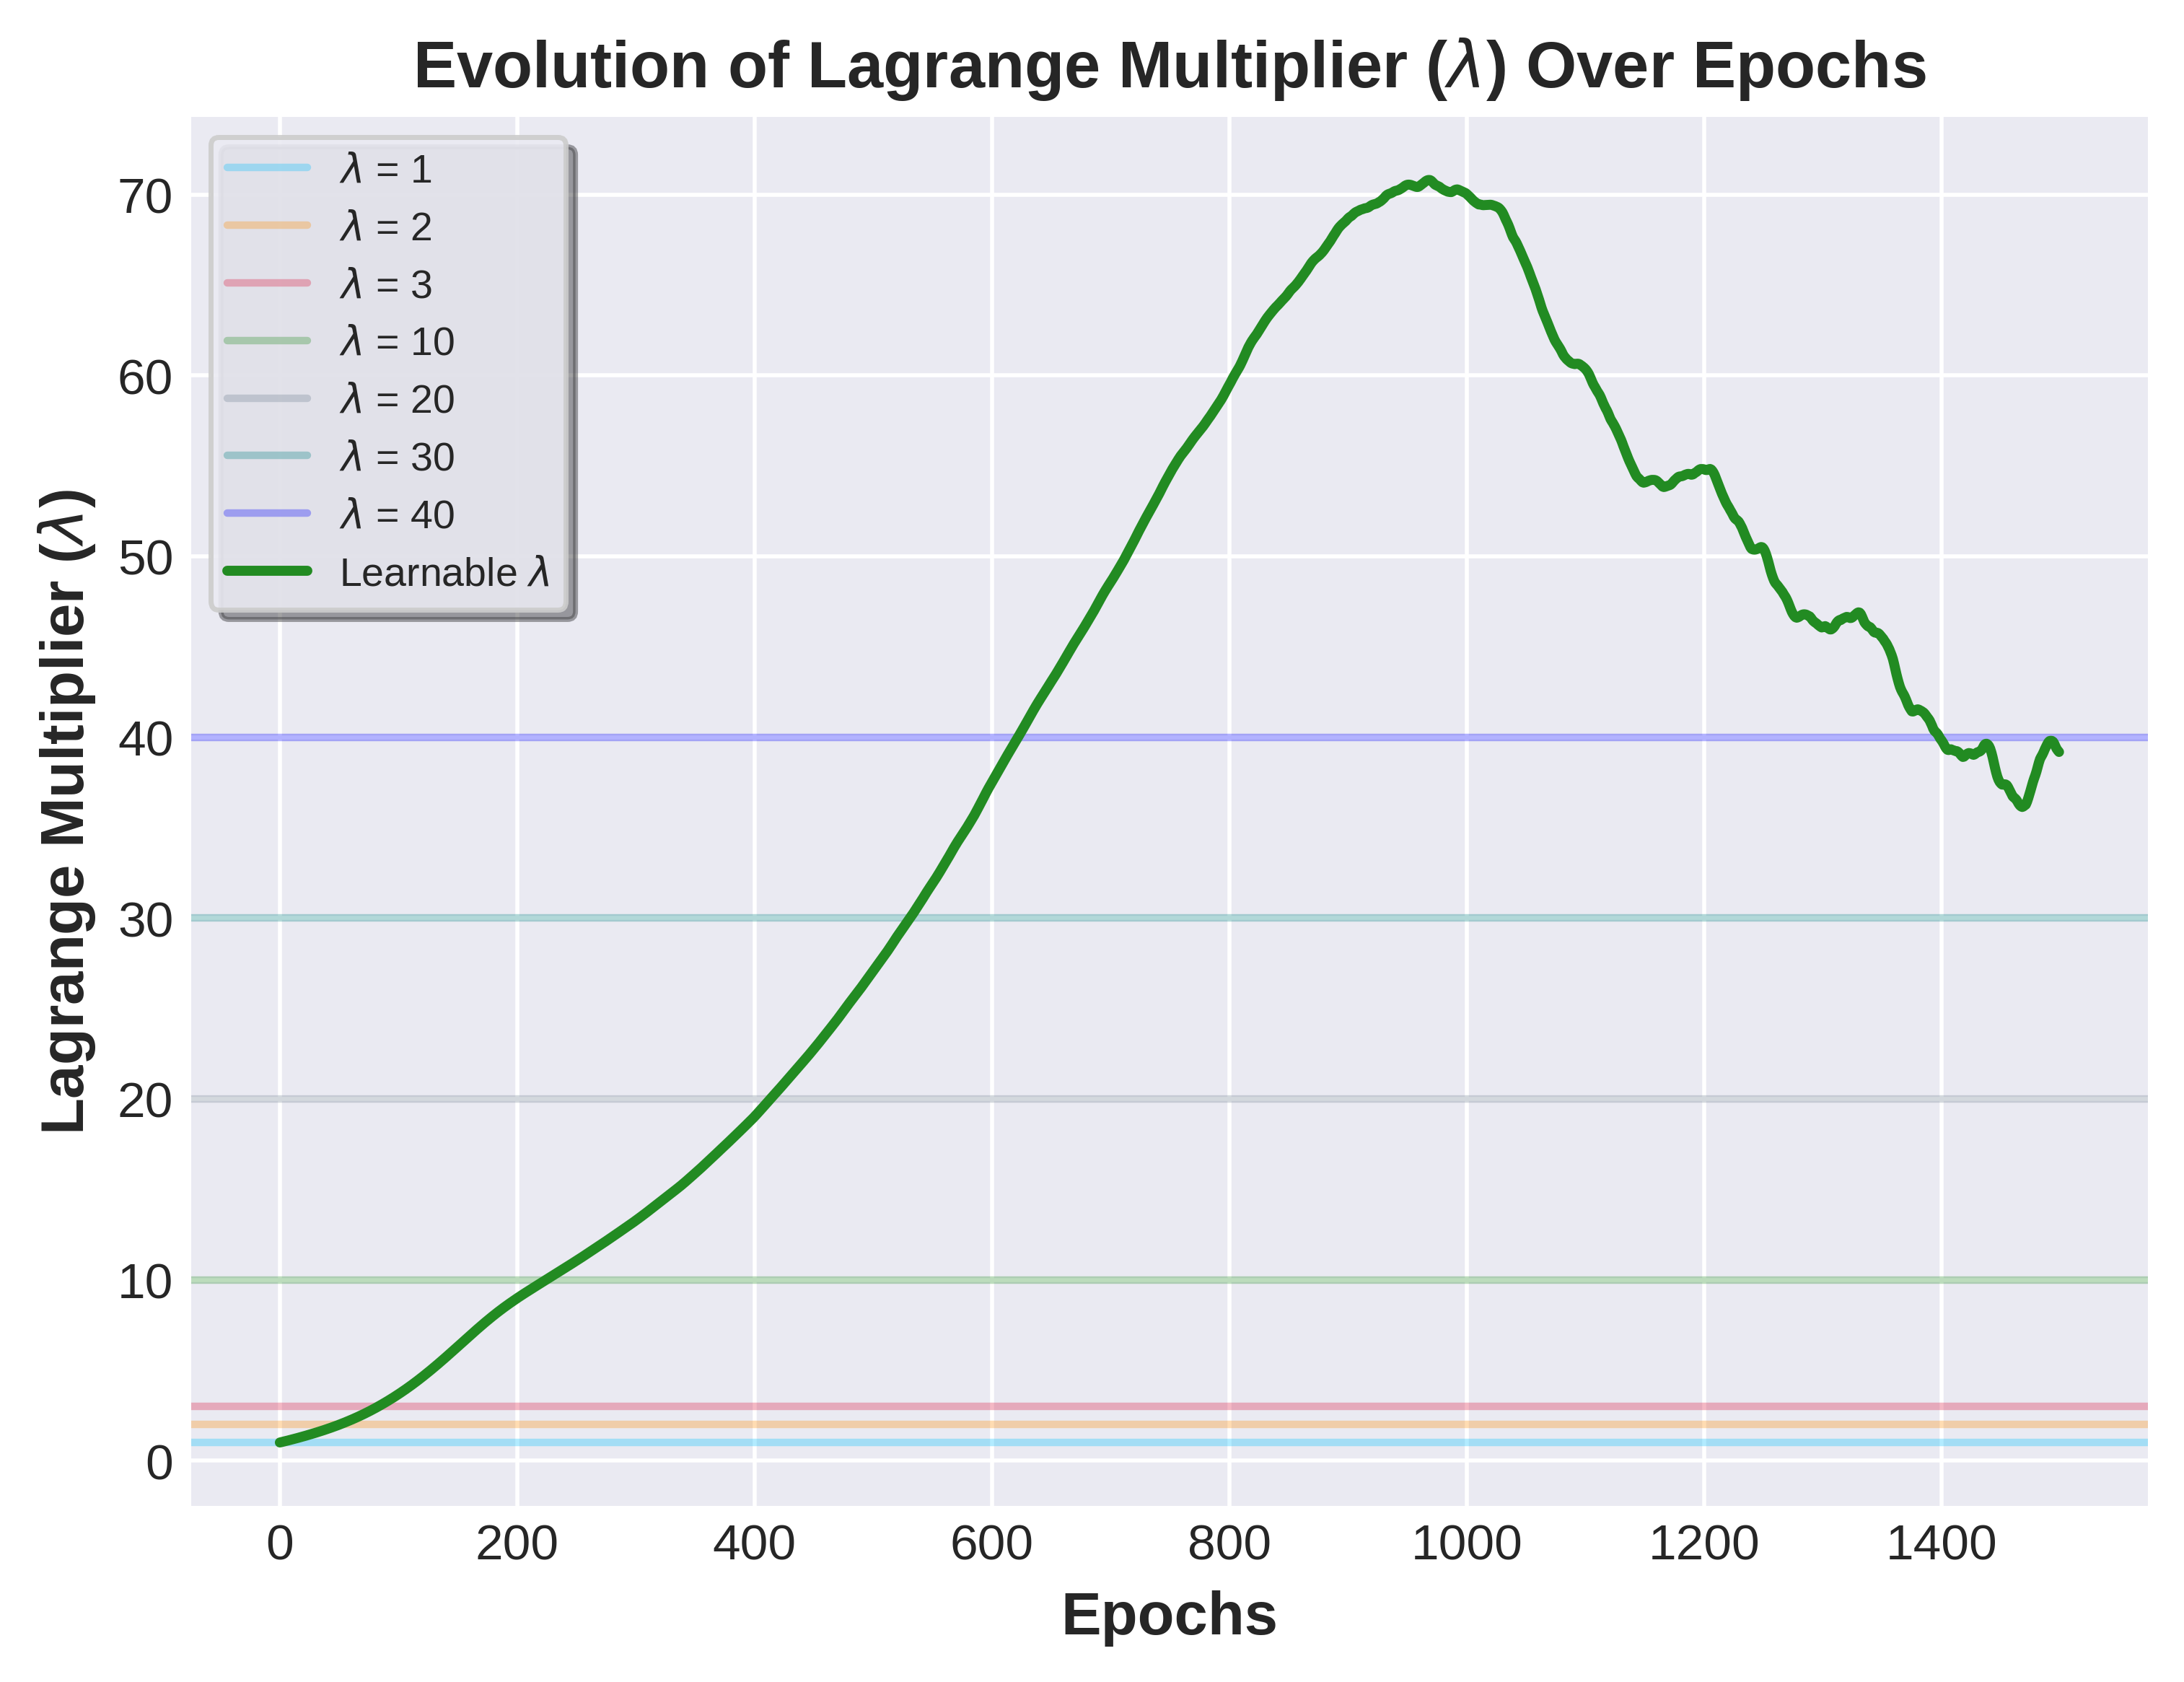
\includegraphics[width=0.32\textwidth]{Images/langragian_multiplier_wo_GECO.png}
			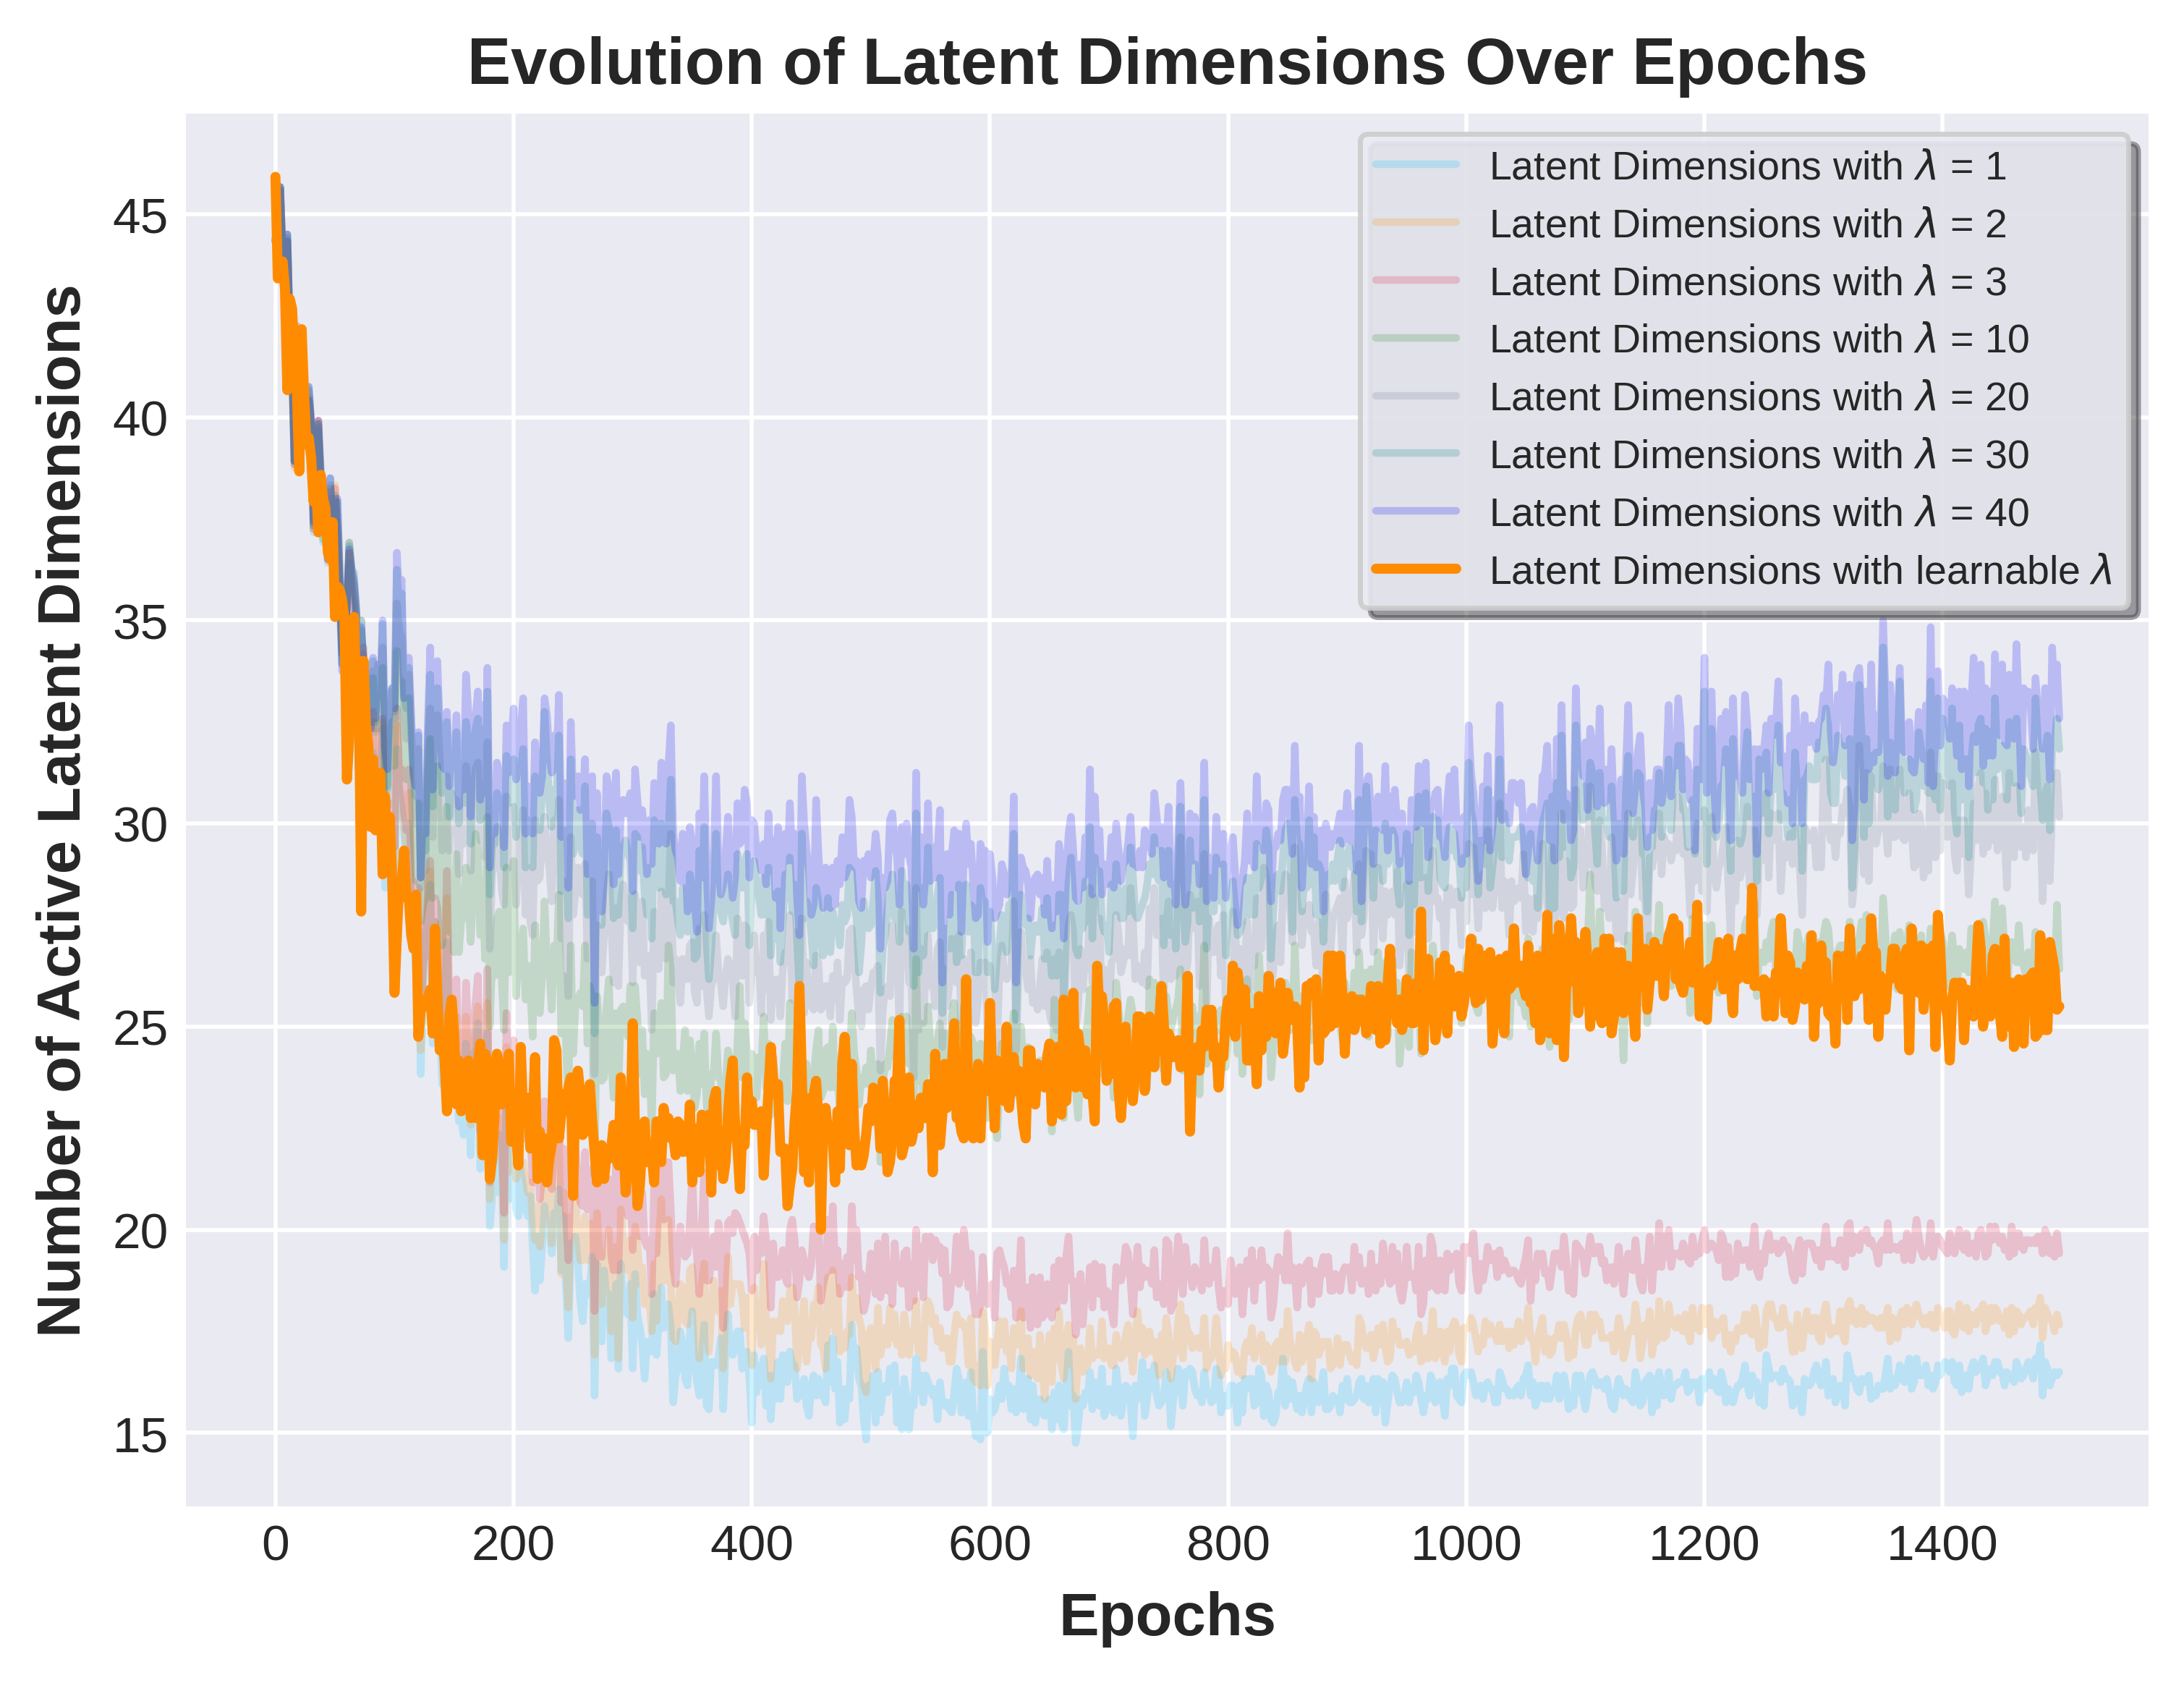
\includegraphics[width=0.32\textwidth]{Images/latent_dims_wo_GECO.png}
			
			
			\caption{Visualization of three key metrics during training: Mean Squared Error (MSE) relative to the threshold $\tau$, the Lagrange multiplier ($\lambda$), and the number of latent dimensions utilized without GECO constraint on prediction task.}
			
			\label{fig:learning_curves_wo_GECO}
			
		\end{figure*}
		content...
	\end{comment}
	
	Table \ref{tab:synthetic} highlights the effectiveness of various methods on a synthetic dataset (8×8×8×$\Omega$), focusing on the ability to estimate treatment effects while identifying and leveraging the true underlying data dimensions. GLOVE-ITE demonstrates it's ability to learn optimal latent representation, achieving the lowest PEHE values: 0.17(0.00), 0.18(0.00), and 0.17(0.027) for $\Omega$=5,10,15, respectively. Importantly, it uses only 26–32 latent dimensions, closely aligning with the actual data regardless of $\Omega$, in contrast to baselines like TEDVAE, TVAE, and DRI-ITE, which rely on significantly larger total dimensionalities (90–120). This dimension efficiency underscores our method’s ability to disentangle relevant features from irrelevant variables while maintaining robust performance. As $\Omega$ increases, GLOVE-ITE effectively adjusts to the true dimensions of the data, showing minimal degradation in PEHE compared to other methods. These results demonstrate the capability of our approach to optimize the use of latent dimensions in variational autoencoders, achieving state-of-the-art accuracy with an efficient and interpretable representation. 
	
	
	
	
	\begin{table}
		\centering
		\caption{Results of the ablation study on the loss function, evaluated on the IHDP dataset with five irrelevant variables. Bold values indicate the best performance (lowest error).}
		\small
		\begin{tabular}{lr}
			\toprule
			Loss & PEHE \\
			\midrule
			
			
			
			%$\mathcal{L}_{\text{ELBO}} + \|\mathbf{m}_{\Gamma, \Delta, \Upsilon,\Omega}\|_0 + \mathcal{L}_{disc}$ (without constraint)     & 1.12(0.60)   	          \\
			$\mathcal{L}_{\text{ELBO}} + \mathcal{L}_{disc}$ 		& 0.81(0.39)    	       \\
			$\mathcal{L}_{\text{ELBO}} + \|\mathbf{m}_{\Gamma, \Delta, \Upsilon,\Omega}\|_0$   	& 0.77(0.40)           \\
			$\mathcal{L}_{\text{ELBO}} + \|\mathbf{m}_{\Gamma, \Delta, \Upsilon,\Omega}\|_0 + \mathcal{L}_{disc}$     	& \textbf{0.75(0.39) }               \\
			$\mathcal{L}_{\text{ELBO}} + \|\mathbf{m}_{\Gamma, \Delta, \Upsilon,\Omega}\|_0 + \mathcal{L}_{disc}+\mathcal{L}_{\mathit{excl}}$    	& \textbf{0.70(0.07) }               \\
			
			\bottomrule
		\end{tabular}
		
		\label{tab:ablation}
		%\todo{The notation here is wrong.}
		
	\end{table}
	\addtocounter{footnote}{+1} %
	
	
	\begin{table}[h]
		\addtolength{\tabcolsep}{-0.5em}
		\centering
		\caption{Compression analysis of the proposed method on synthetic data with an 8×8×8×5 dimensional structure, evaluated under varying initial dimensionality settings. }
		\small
		\begin{tabular}{rrrrrr}
			\toprule
			Initial\_dimensions& $\Gamma$-dims & $\Delta$-active & $\Upsilon$-active & $\Omega$-active & Total-active \\
			\midrule
			
			60         	& 8 & 9      & 8   & 6            & 31            \\
			68         	& 7 & 8      & 8  & 5            & 28            \\
			76         	& 5 & 9      & 9   & 6          & 29            \\
			84         	& 9 & 7      & 8    & 5          & 29            \\
			
			
			\bottomrule
		\end{tabular}
		
		\label{tab:compression}
	\end{table}
	
	\begin{figure*}
		\centering
		%\captionsetup{justification=centering}
		
		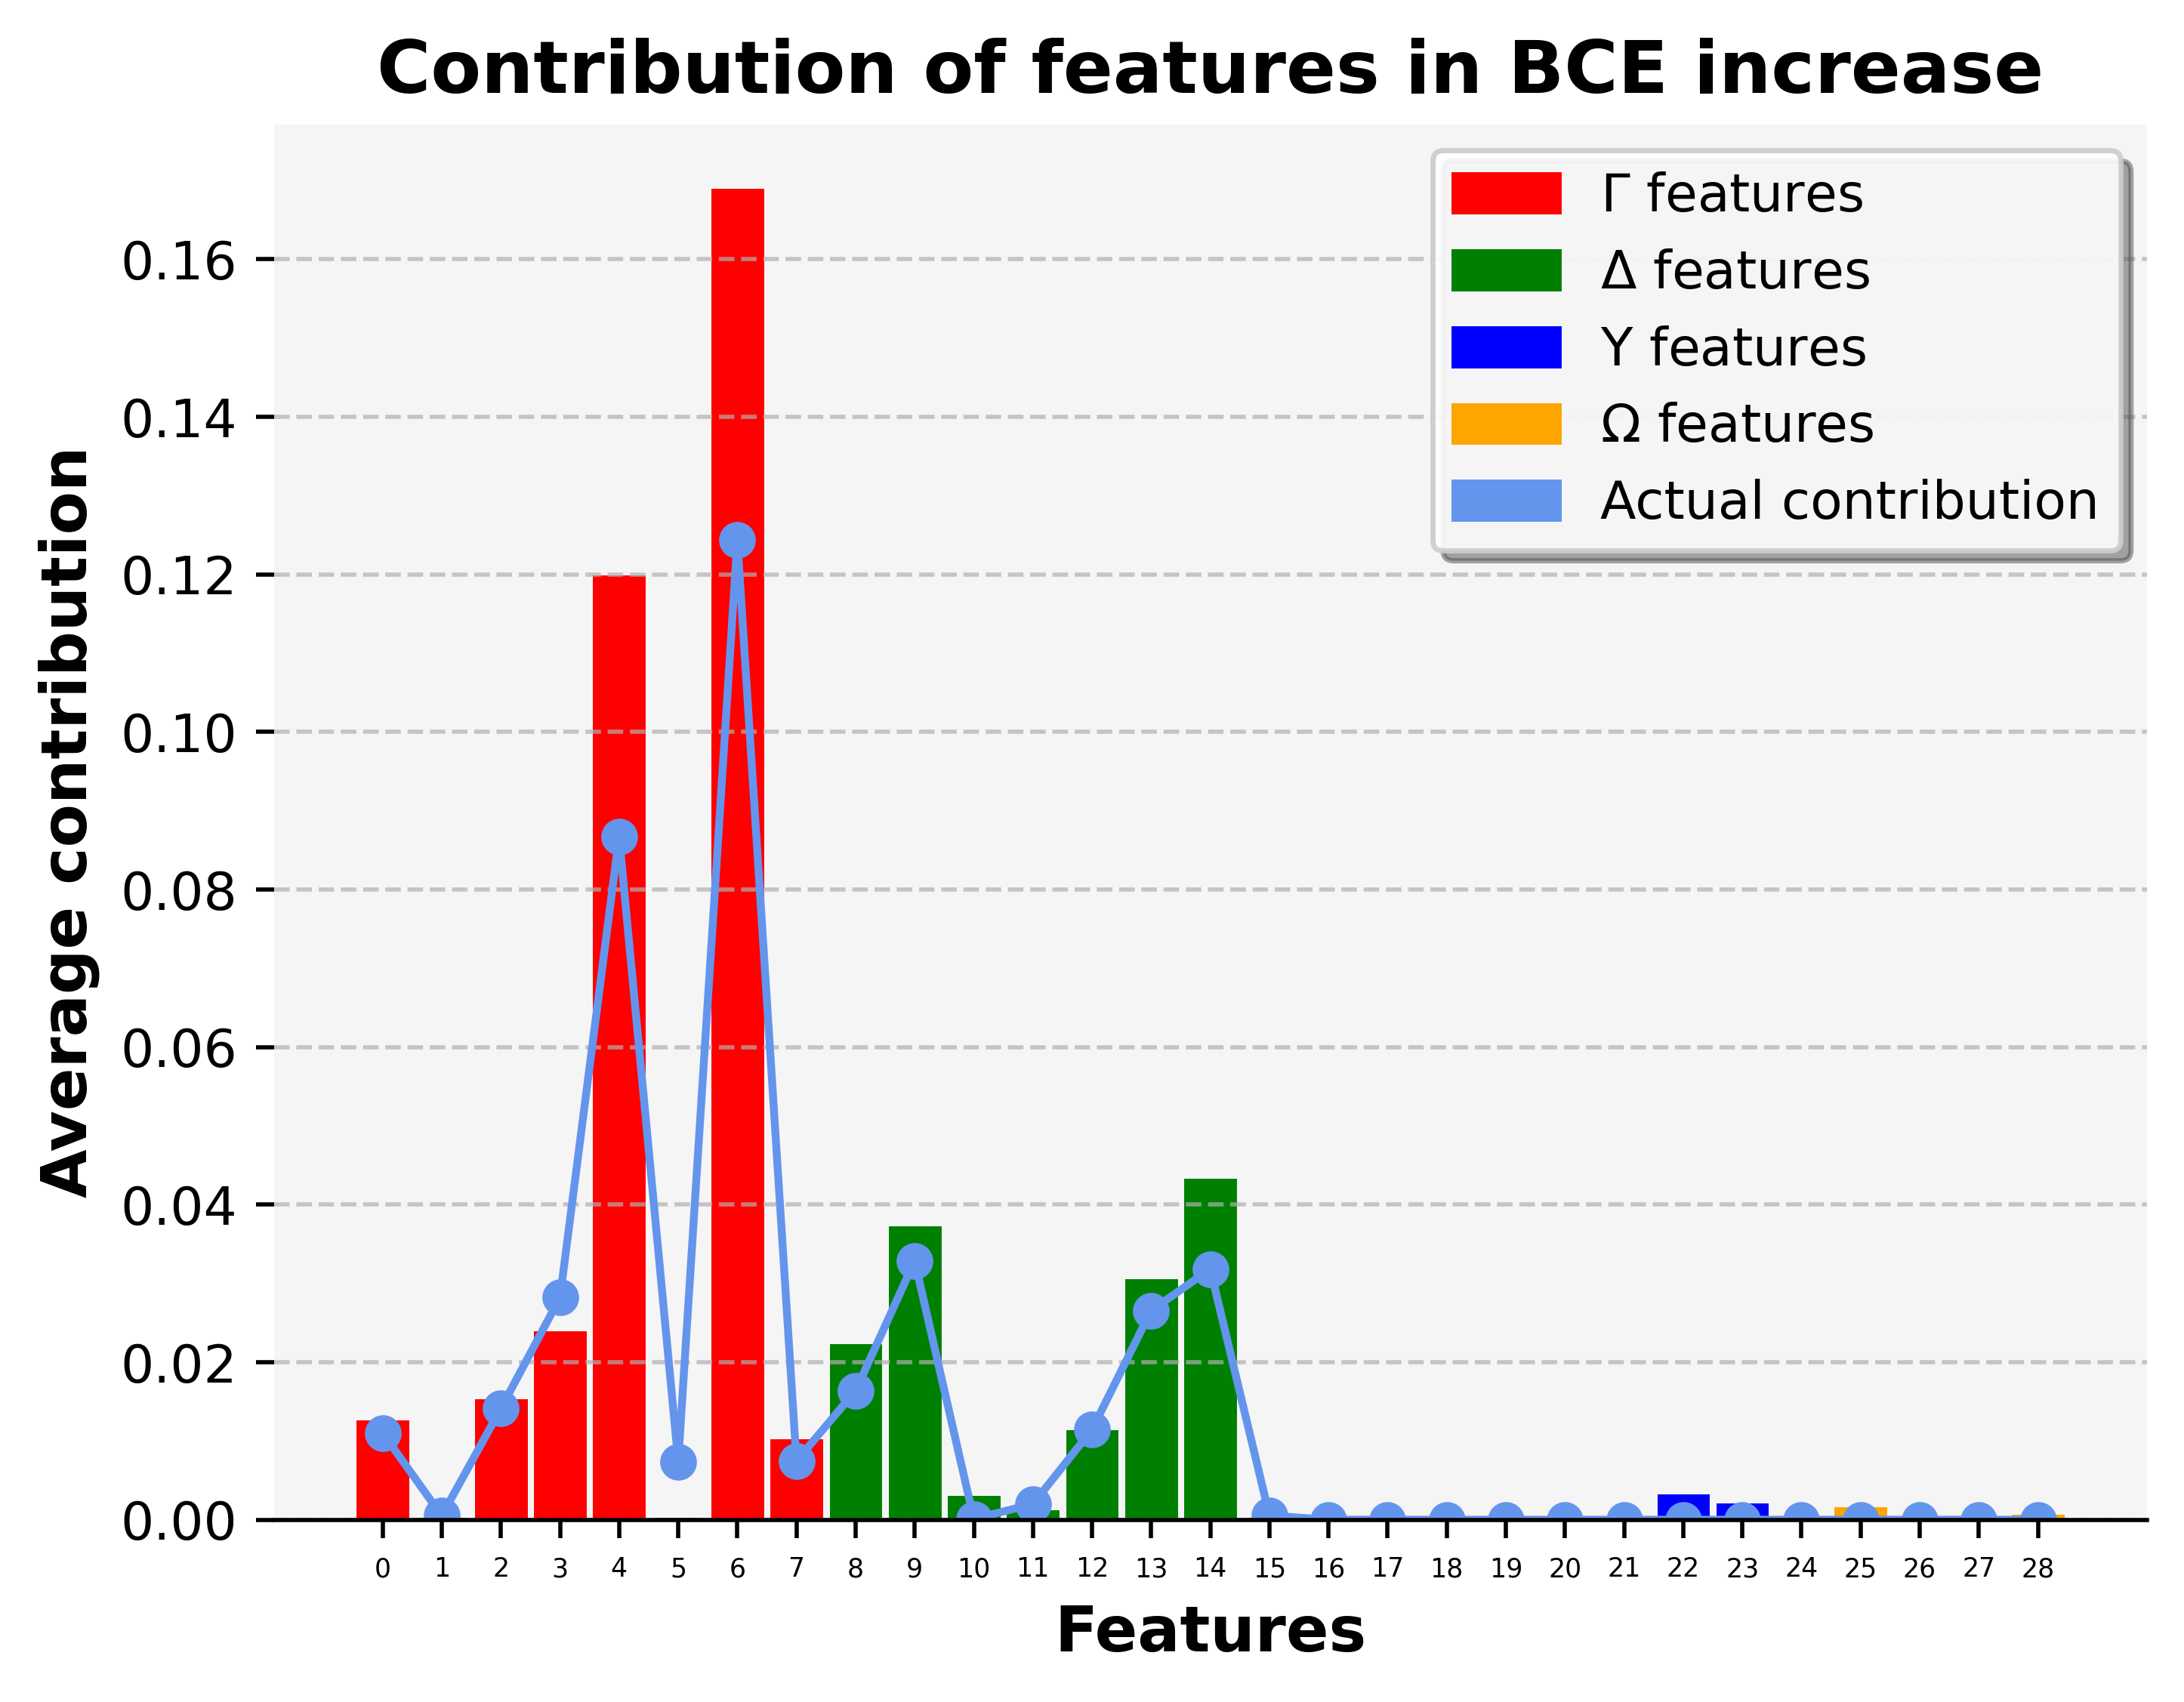
\includegraphics[width=0.33\textwidth]{Images/bce_increase.png}
		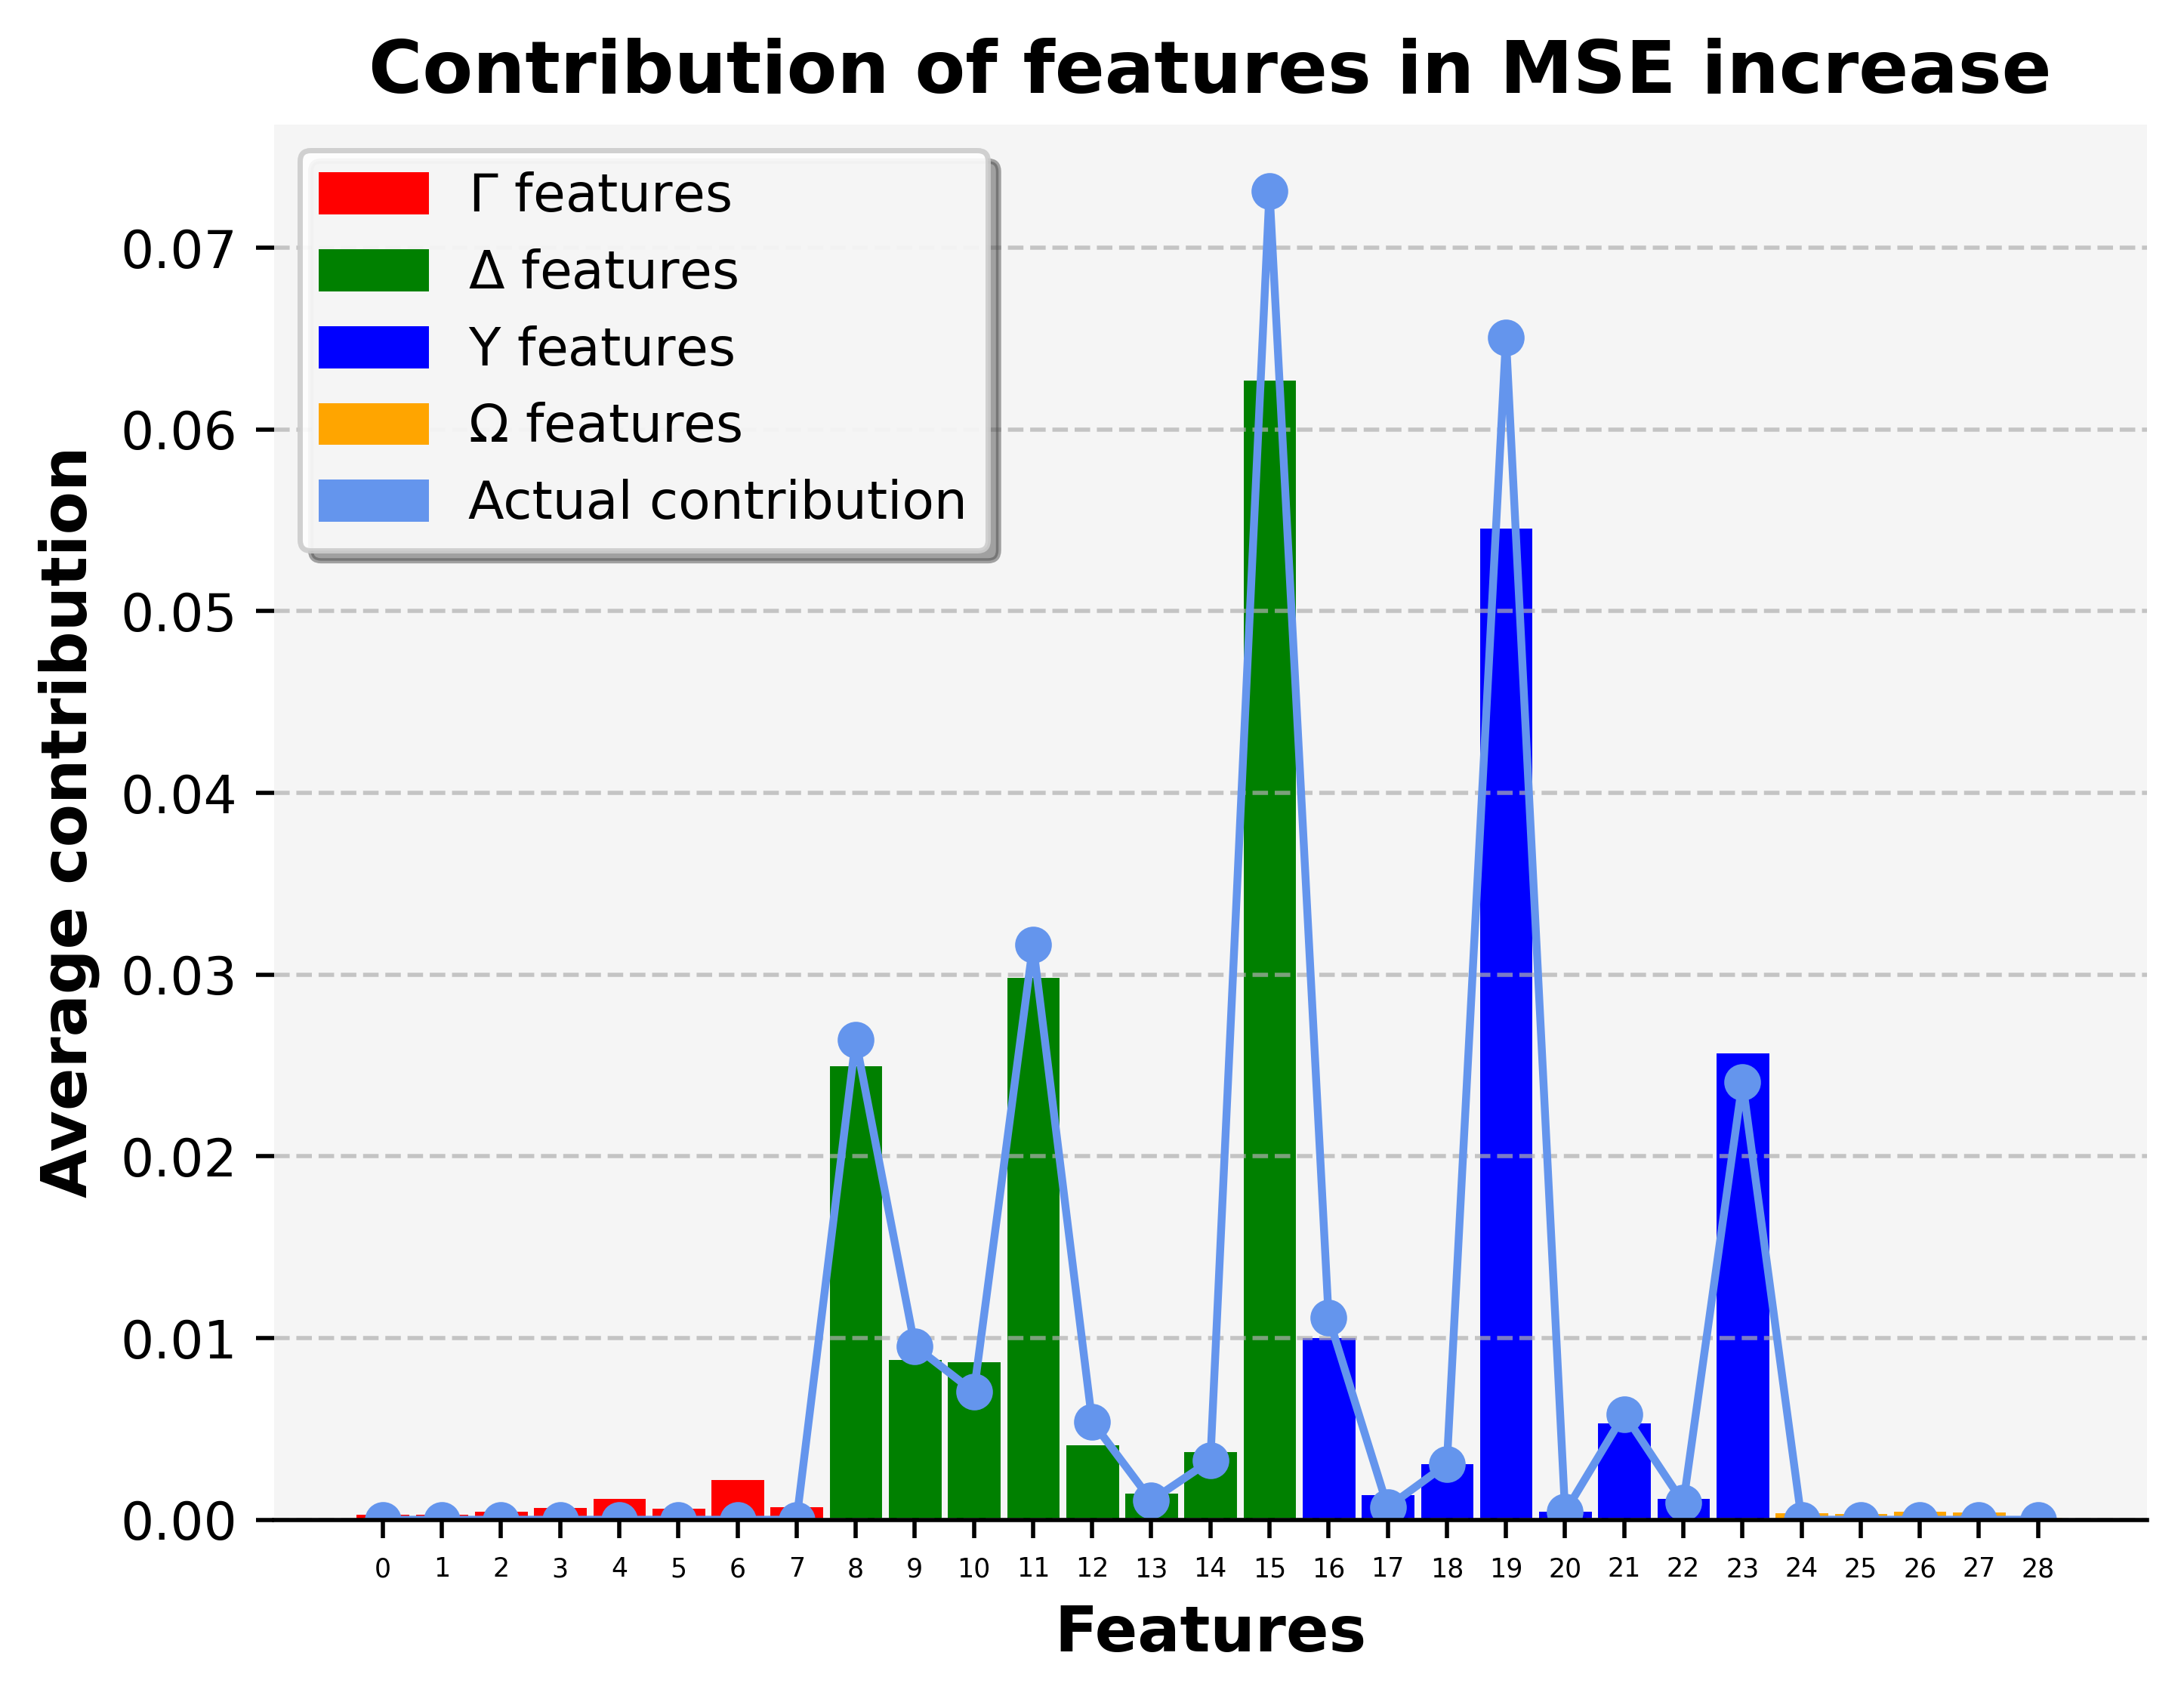
\includegraphics[width=0.33\textwidth]{Images/mse_increase.png}
		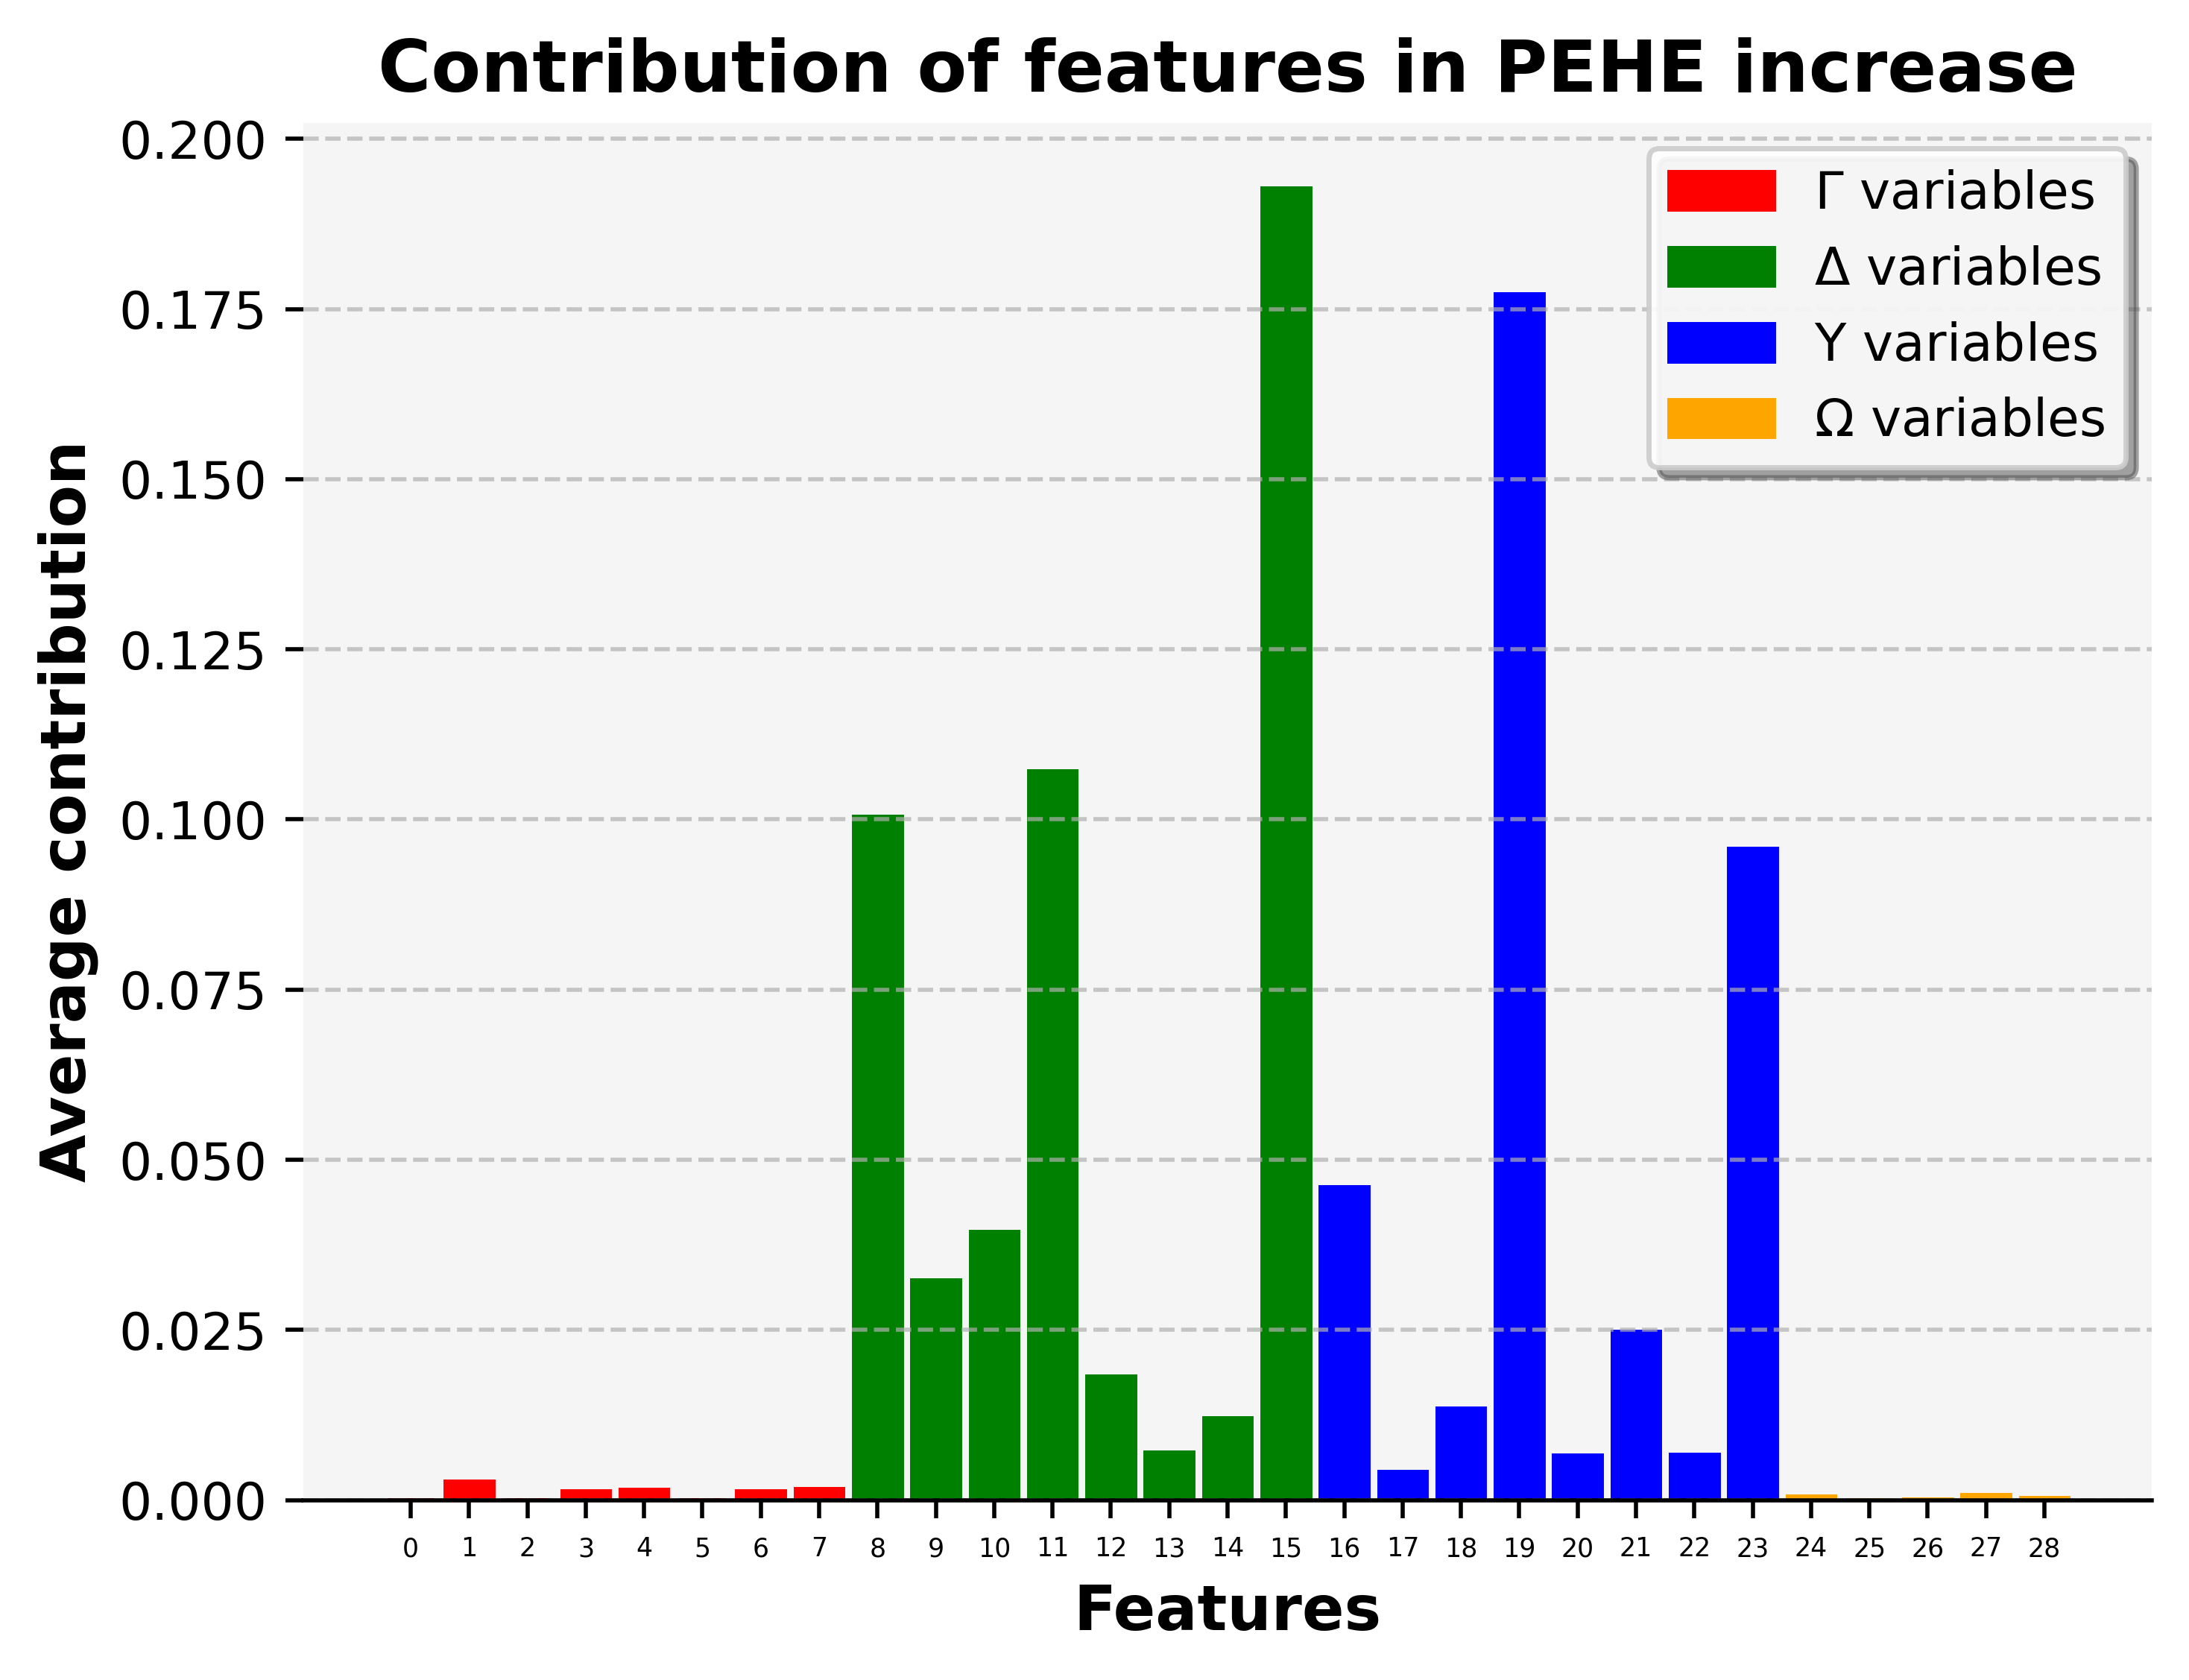
\includegraphics[width=0.33\textwidth]{Images/pehe_increase.png}
		
		
		\caption{Feature permutation analysis demonstrating the inference and disentanglement of latent across BCE, MSE, and PEHE tasks.}
		
		\label{fig:permutation}
		
	\end{figure*}
	
	\subsection{Qualitative Evaluation of Model Performance}
	
	Figure \ref{fig:learning_curves} illustrates the learning dynamics of our model, focusing on three key quantities: (1) Mean Squared Error Constrained (MSEC), (2) the Lagrange multiplier ($\lambda$), and (3) the number of active latent dimensions during training. To ensure stability and a reliable estimate, we show the average of the last five active dimension values after each epoch instead of the final value alone. Early in training, the $L_0$ regularizer aggressively reduces the number of active latent dimensions, causing an initial rise in MSEC around the 200$^{th}$ epoch. Simultaneously, $\lambda$ increases steadily to enforce the MSE constraint. As training progresses, the MSEC gradually decreases toward the specified tolerance ($\tau$), while the number of active latent dimensions increases to balance dimensional efficiency with predictive accuracy. By the end of training, the MSEC stabilizes near $\tau$, the number of active dimensions converges, and $\lambda$ reaches a stable value, indicating successful convergence. Notably, models with fixed $\lambda$ fail to achieve comparable results, struggling to balance the trade-off between the two objectives effectively. 
	
	
	
	
	\textbf{Ablation study:} Table \ref{tab:ablation} summarizes an ablation study evaluating the impact of different components of the loss function on PEHE performance using the IHDP dataset with five irrelevant variables. Combining the ELBO, masks ($L_0$ regularization) and the dicrepancy loss without enforcing the MSE constraint performs worse, with a PEHE of 1.12(0.60), indicating the necessity of constraint enforcement. Adding the discrepancy loss ($\mathcal{L}_{disc}$) alongside ELBO but without masks ( $L_0$ regularization) results in a lower PEHE of 0.81(0.39). Further, removing only the discrepancy loss achieves PEHE of 0.77 (0.40). The complete loss function, integrating ELBO, masks ($L_0$ regularization), discrepancy loss, and the MSE constraint, achieves the best PEHE of 0.75(0.39), demonstrating the importance of a balanced combination of these components for optimal performance.
	
	
	
	\textbf{Compression analysis:} Table \ref{tab:compression} presents a compression analysis of the proposed method on synthetic data with an 8×8×8×5 dimensional structure, evaluated across varying initial dimensionality settings. Despite starting with different initial dimensions (ranging from 60 to 84), the method consistently compresses the data to a compact latent representation, utilizing only 29–31 total dimensions. This highlights the model's ability to adaptively allocate dimensions among $\Gamma,\Delta$,$\Upsilon$ and $\Omega$ encoders, with minor variations depending on the initial input size. For instance, with initial dimensions of 76 or 84, the method converges to 29 latent dimensions, while for 60 and 68, it stabilizes at 31 and 28 dimensions. These results emphasize the model's robustness in achieving efficient compression irrespective of the initial input dimensionality, while preserving the underlying data structure.
	
	
	
	\textbf{Inference and Disentanglement:}
	
	Figure \ref{fig:permutation} highlights the inference of latent factors using the permutation feature importance theory \citep{Fisher,Khan2024OnTE}. Specifically, it demonstrates that only $\Gamma$ and $\Delta$ features contribute to an increase in the BCE loss, validating our method's ability to accurately infer these factors within the data.
	
	\begin{figure}[h]
		\centering
		%\captionsetup{justification=centering}
		
		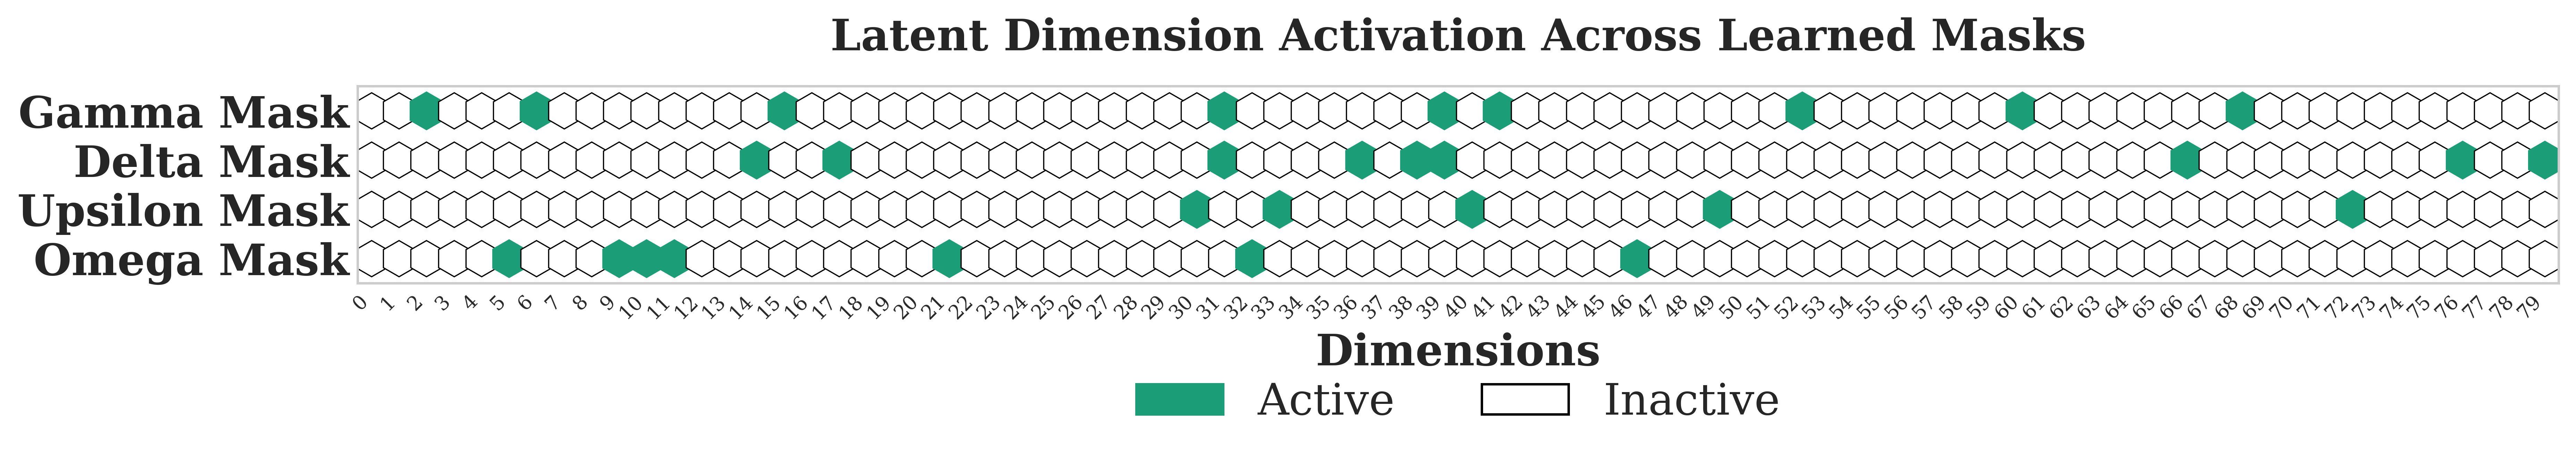
\includegraphics[width=0.5\textwidth]{Images/orthogonal.png}
		
		\caption{Four learned masks showing active (green) and inactive (white) latent dimensions. Each mask activates distinct subsets of latent dimensions with minimal overlap—only one dimension is shared across all masks (visible as green in a single column)—indicating that the masks are learning largely independently. The observed overlap is just 2.5\%, highlighting the natural disentanglement effect of integrating sparsity-inducing masks within the VAE framework.}
		
		.
		%\todo[author=jsk]{I do not know if this result id good or bad. Should we not have zero overlap in a correct causal model? Is there any way to show how much overlap there would be if we did not have masks. Do we make clear enough that minimal overlap is not a training objective but a side-effect?}
		
		
		\label{fig:ortho}
		
	\end{figure}
	
	\begin{figure}[h]
		\centering
		%\captionsetup{justification=centering}
		
		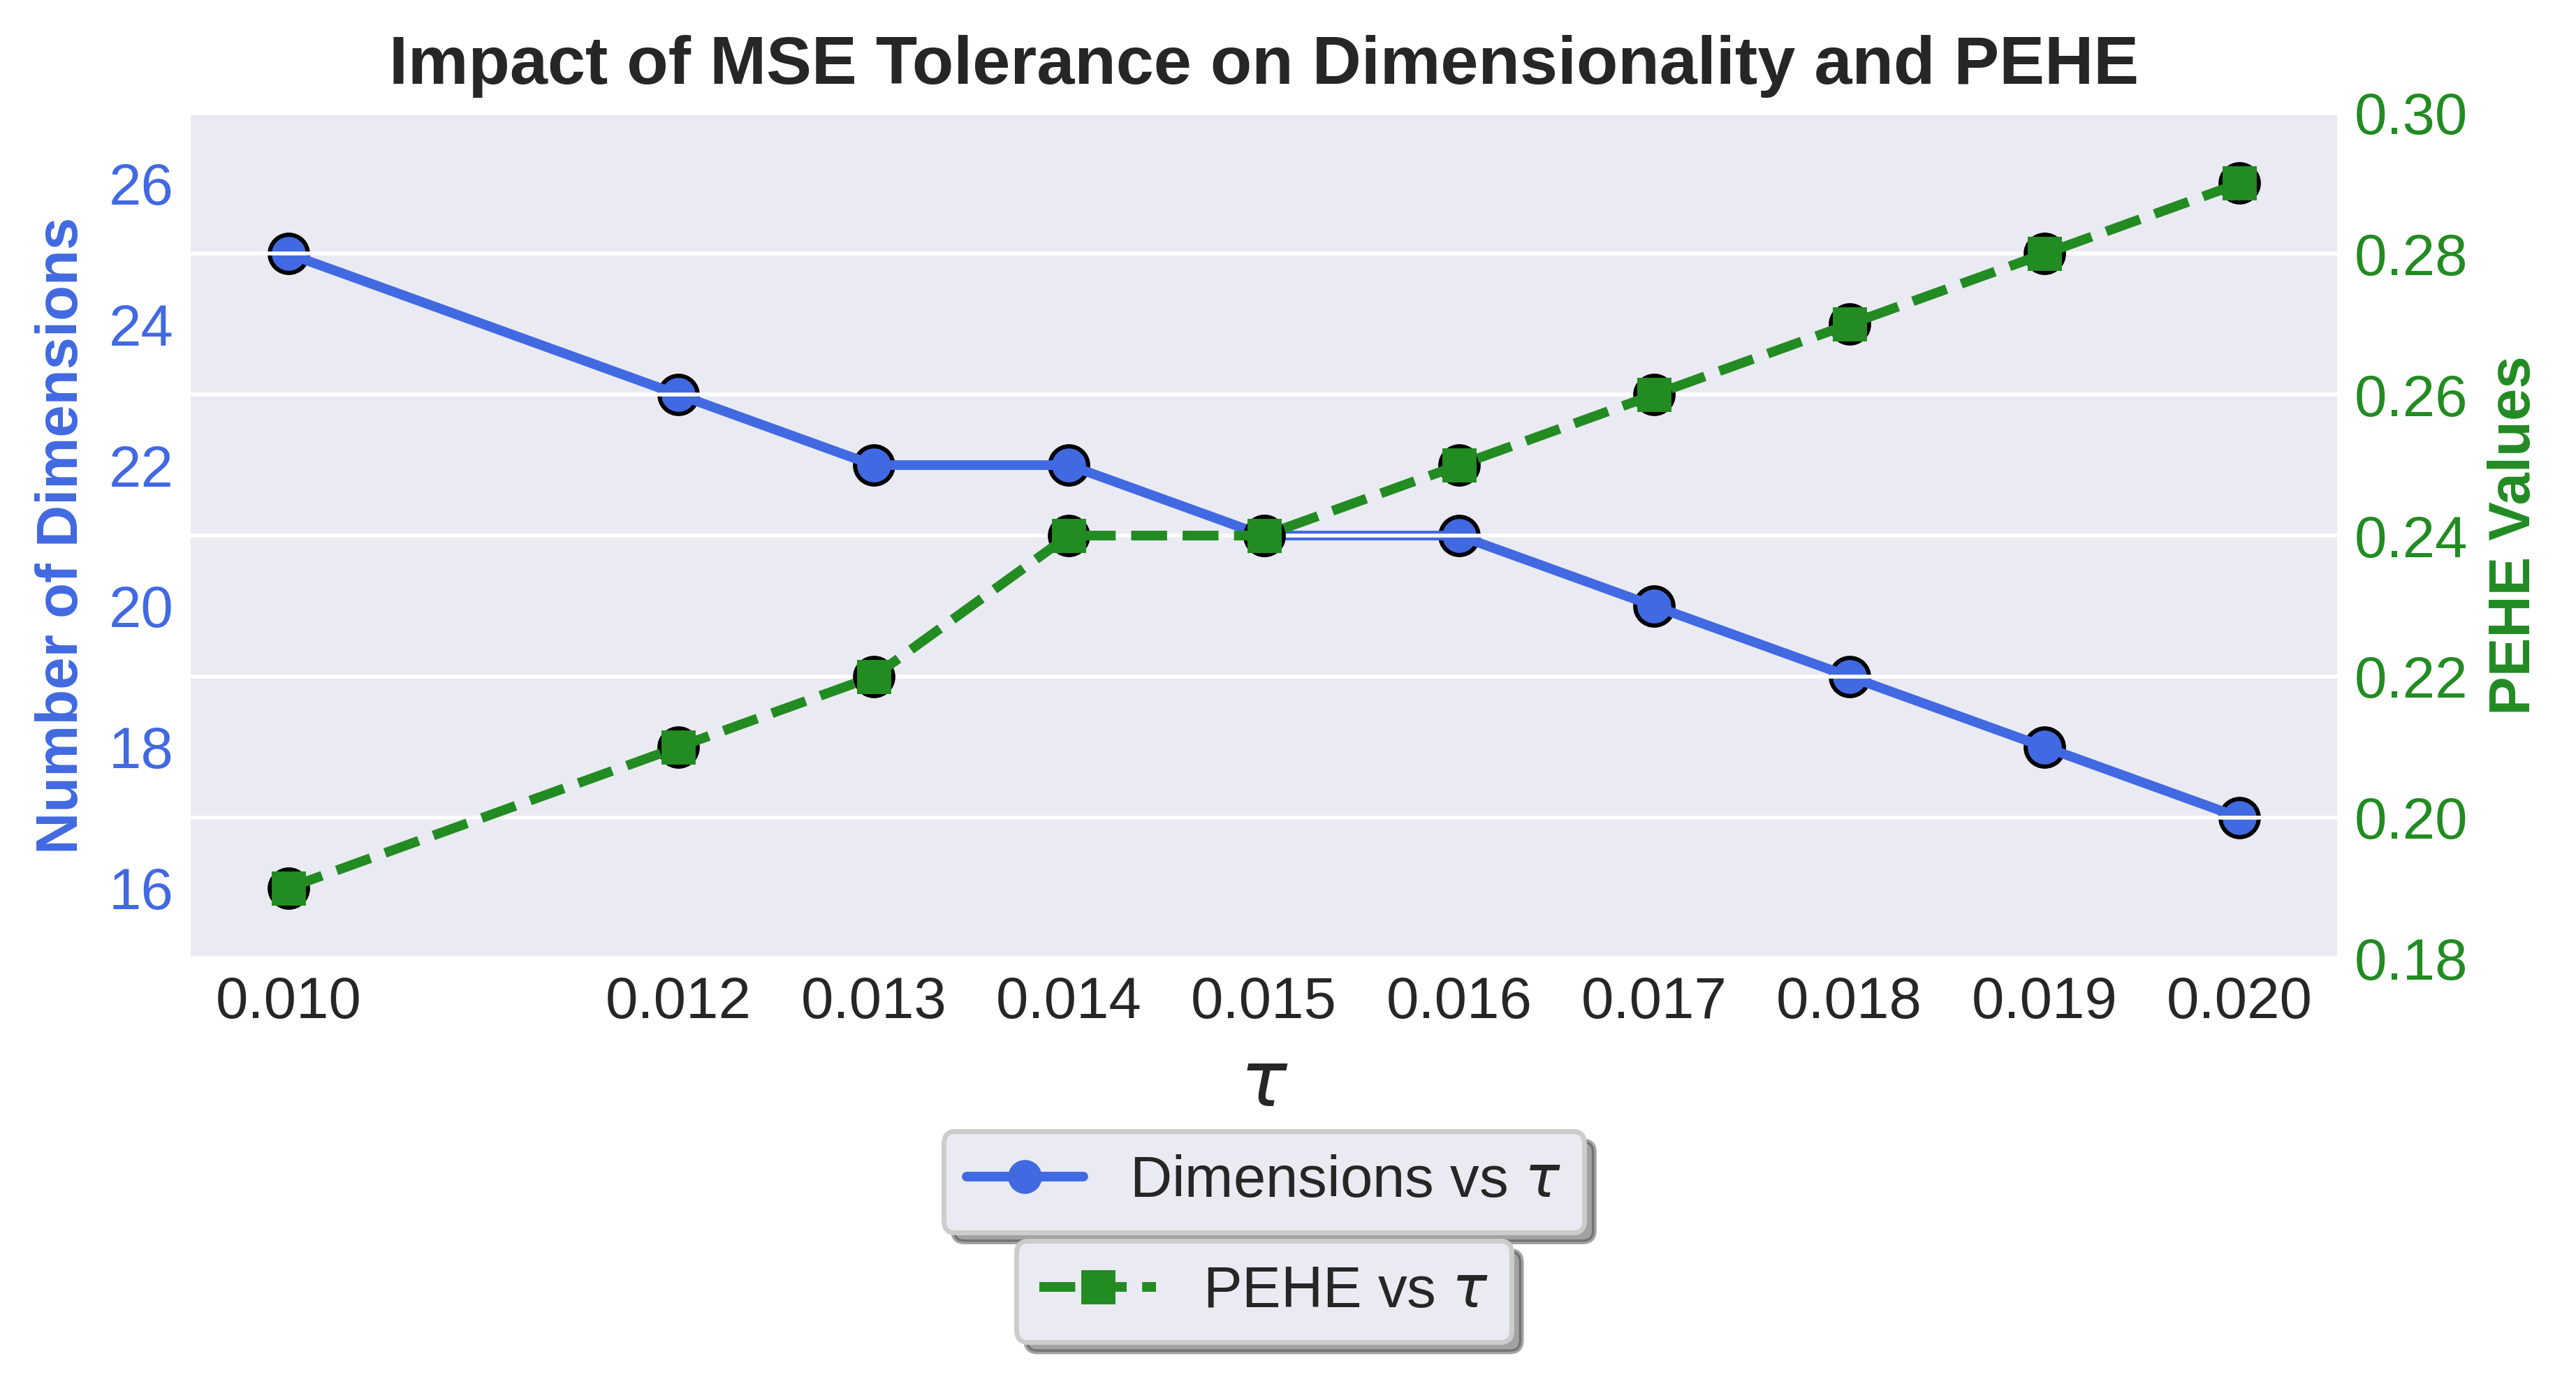
\includegraphics[width=0.47\textwidth]{Images/tol_vs_dims_pehe.png}
		
		
		
		\caption{Visualization of active dimensionality and PEHE as functions of MSE tolerance.}
		
		\label{fig:tolerance}
		
	\end{figure}
	
	Similarly, it confirms the successful learning of $\Delta$ and $\Upsilon$ factors, as evidenced by their impact on the MSE when permuted. Finally, it illustrates that GLOVE-ITE effectively disentangles and infers $\Omega$, as permuting irrelevant features does not affect the PEHE, while permuting relevant features leads to a significant increase. This comprehensive analysis underscores the robustness of GLOVE-ITE in inferring and disentangling the critical latent factors. \citet{CEVAE,lowe2022amortized} show that when latent factors are correctly inferred, causal effects can be identified and the reliance on the ignorability (unconfoundedness) assumption is reduced \citep{vowels2021targeted}.
	
	
	%\textbf{Identification and disentanglement:} Figure \ref{fig:permutation} highlights the identification of latent factors using the permutation feature importance theory \cite{Fisher,Khan2024OnTE}. Specifically, it demonstrates that only $\Gamma$ and $\Delta$ features contribute to an increase in the BCE loss, validating our method's ability to accurately identify these factors within the data. Similarly, it confirms the successful identification of $\Delta$ and $\Upsilon$ factors, as evidenced by their impact on the MSE when permuted. Finally, it illustrates that GLOVE-ITE effectively disentangles and identifies $\Omega$, as permuting irrelevant features does not affect the PEHE, while permuting relevant features leads to a significant increase. This comprehensive analysis underscores the robustness of GLOVE-ITE in identifying and disentangling the critical latent factors.%
	
	
	
	\textbf{Tolerance ($\tau$) effect:} Figure \ref{fig:tolerance} highlights the relationships between MSE tolerance ($\tau$), the number of active latent dimensions, and PEHE. The figure clearly shows that $\tau$ is inversely related to the number of active dimensions—higher tolerances result in fewer dimensions. Conversely, MSE tolerance has a direct relationship with PEHE, as increasing the $\tau$ leads to higher estimation errors. This trade-off highlights the importance of selecting an appropriate tolerance level to balance computational efficiency and estimation accuracy. 
	
	
	\section{Conclusion}
	
	In this work, we proposed a novel VAE-based framework that integrates the Generalized ELBO with Constrained Optimization (GECO) and an L$_0$ sparsity objective to address the challenge of determining the effective latent size in treatment effect estimation. Our method learns compact and disentangled latent representations, enabling both interpretability and computational efficiency. Through extensive evaluation, we demonstrate that it consistently outperforms state-of-the-art baselines in terms of predictive accuracy and robustness, particularly in high-dimensional settings with many irrelevant variables.
	
	
	\begin{comment}
		tackle the challenges of treatment effect estimation. Our approach addresses the critical issue of determining the latent dimensionality by dynamically learning a sparsity mask, ensuring robust disentanglement and compliance with the prediction task constraints.
		
		Through comprehensive experiments on the IHDP and synthetic datasets, we demonstrated that our method outperforms existing state-of-the-art approaches, offering superior accuracy, faster convergence, and improved scalability. By utilizing a unified encoder design, we eliminated the need for additional encoders to handle irrelevant variables, enhancing both computational efficiency and representation learning quality.
		
		The proposed framework not only advances the state of the art in treatment effect estimation but also provides valuable insights into optimizing latent space representations for broader applications.
		content...
	\end{comment}
	%%%%%%%%%%%%%%%%%%%%%%%%%%%%%%%%%%%%%%%%%%%%%%%%%%%%%%%%%%%%%%%%%%%%%%%%
	
	%%% Use this environment to include acknowledgements (optional).
	%%% This will be omitted in doubleblind mode.
	
	\begin{ack}
		By using the \texttt{ack} environment to insert your (optional) 
		acknowledgements, you can ensure that the text is suppressed whenever 
		you use the \texttt{doubleblind} option. In the final version, 
		acknowledgements may be included on the extra page intended for references.
	\end{ack}
	
	%%%%%%%%%%%%%%%%%%%%%%%%%%%%%%%%%%%%%%%%%%%%%%%%%%%%%%%%%%%%%%%%%%%%%%%%
	
	%%% Use this command to include your bibliography file.
	
	\bibliography{mybibfile}
	
\end{document}
%%%%%%%%%%%%%%%%%%%%%%%%%%%%%%%%%%%%%%%%%%%%%%%%%%%%%%%%%%%%%%%%%%%%%%